\documentclass[a4paper,11pt]{report} % ligne de classe
% preambule

\usepackage[utf8]{inputenc}
\usepackage[T1]{fontenc}
\usepackage[frenchb]{babel}
\usepackage{textcomp} 
\usepackage[top=3cm,left=3cm,right=3cm,bottom=2cm]{geometry}
\usepackage{lmodern}
\usepackage{sectsty}
%\usepackage{nicefrac}
\usepackage{graphicx}
\usepackage{lastpage}
\usepackage{fancyhdr}
\usepackage{amsmath}
\usepackage{amssymb}
\usepackage{amsfonts}
\usepackage{capt-of}
\usepackage{caption}
\usepackage{tikz}
\usepackage{multirow}
\usepackage{bm}
\usepackage{mathtools}
    
    
\usepackage{fancyvrb} % pour forcer les verbatim sur une seule page
\usepackage{url}
    
%\usepackage{subfigure}
\usepackage{subcaption}
    
%\newcommand\matlab{MATLab\textsuperscript{\textregistered}}

\renewcommand{\baselinestretch}{1.1}
\newcommand{\dd}{\partial}
\newcommand{\tr}[1]{\prescript{t\hspace{-0.08cm}}{}{#1}}


\usepackage[colorinlistoftodos]{todonotes}

%\usepackage{cite} 
\usepackage[round,authoryear,numbers]{natbib}


\usepackage{hyperref}
\hypersetup{
     colorlinks   = true,
     citecolor    = blue!90
}

%numerotation des lignes (pour la relecture)
\usepackage{lineno} 



\begin{document} % début du doc
% corps du doc

\begin{titlepage}

\newcommand{\HRule}{\rule{\linewidth}{0.5mm}} % Defines a new command for the horizontal lines, change thickness here

\center % Center everything on the page
 
%----------------------------------------------------------------------------------------
%	HEADING SECTIONS
%----------------------------------------------------------------------------------------

\textsc{\large Université du Maine \\ UFR Sciences et Techniques}\\[0.5cm] % Name of your university/college

\textsc{ \large Master Acoustique 2\textsuperscript{ème} année}\\[3.0cm] % Major heading such as course name
\textsc{\Large Rapport de Stage}\\[0.5cm] % Minor heading such as course title

%----------------------------------------------------------------------------------------
%	TITLE SECTION
%----------------------------------------------------------------------------------------

\HRule \\[0.7cm]
{ \huge \bfseries Imagerie ultrasonore par inversion de formes d'onde}\\[0.4cm] % Title of your document
\HRule \\[1.5cm]
 
%----------------------------------------------------------------------------------------
%	AUTHOR SECTION
%----------------------------------------------------------------------------------------


{\Large Alice \textsc{Dinsenmeyer}}\\[3cm]

\Large encadrée par : \\[1cm]
Romain \textsc{Brossier} et
Ludovic \textsc{Moreau}\\
Maîtres de conférence, ISTerre

% If you don't want a supervisor, uncomment the two lines below and remove the section above
%\Large \emph{Author:}\\
%John \textsc{Smith}\\[3cm] % Your name

%----------------------------------------------------------------------------------------
%	DATE SECTION
%----------------------------------------------------------------------------------------
\vfill
{\large Année universitaire 2015-2016}\\[3cm] % Date, change the \today to a set date if you want to be precise
 


%----------------------------------------------------------------------------------------
%	LOGO SECTION
%----------------------------------------------------------------------------------------
\begin{minipage}{0.3\textwidth}
	\centering
	
\includegraphics[height=2.5cm]{img/univ.png}	
\end{minipage}
\begin{minipage}{0.3\textwidth}
	\centering	
	
\includegraphics[height=2.5cm]{img/cnrs.jpg}
\end{minipage}
\begin{minipage}{0.3\textwidth}
	\centering
	
\includegraphics[height=2.5cm]{img/isterre.jpg}
\end{minipage}
 % Include a department/university logo - this will require the graphicx package

 


%----------------------------------------------------------------------------------------
%\vfill % Fill the rest of the page with whitespace

\end{titlepage}


\newpage
%\section*{Remerciements}





\vspace{2cm}
%\section*{Abstract}

Weld imaging is crucial to control health of cooling systems and pipeline. But methods currently used do not take well into account the strong anisotropy induced by grain structure of welds. The time shift caused by anisotropy cannot be predicted and thus, defects in weld cannot be localised precisely. \\

The full waveform inversion (FWI) attempts to build an image of elastic parameters and hence could take accurately into account anisotropic propagation. It is based on an optimisation problem that aims to reduce the misfit between recorded and computed data by perturbing the model parameters. \\

A study of resolution shows that FWI can provide high resolution image depending on the acquisition system, the records duration and the scattering pattern of the different parameters. Some applications of time-domain FWI to 2D-acoustic welds are performed under isotropic and transversal isotropic propagation approximation. When each isotropic parameter is inverted independently of the other one, wrong high frequency perturbations are introduce in the velocity model. It is due to leakage of the density perturbations over the velocity parameter. Moreover, the density parameter is poorly reconstructed, because its effect on the observed data is weaker. Multiparametric FWI is challenging because it increases ill-posedness of the inversion, but it improves the velocity reconstruction, by reducing the high frequency artefacts. In the transverse isotropic case, it appears that surface acquisition makes horizontal velocity hard to build, even with wide azimuthal data. 

%t affects more weakly the observed data.





 %Moreover, multiparametric FWI, which is challenging because it increases ill-posedness of the inversion, 


%\smallskip \textbf{Mot-clés} : ECND par ultrasons, problèmes d'optimisation,  

%\tableofcontents

%\addcontentsline{toc}{section}{\textbf{Introduction}}
\chapter*{Introduction}

Dans l'industrie ou le domaine médical, il est nécessaire de connaître les propriétés et contrôler l'évolution de matériaux élastiques. Pour cela, en complément des ondes électromagnétiques,  les ondes ultrasonores sont utilisées en raison de leur plus faible atténuation.\\~\\

Le contrôle non-destructif (CND) de soudures a des enjeux majeurs en terme de sécurité. Une bonne qualité d'image est indispensable pour contrôler l'évolution des soudures de structures critiques, telles que les systèmes de refroidissement de centrale nucléaire ou les canalisations pour le transport de matières fluides (hydrocarbure, gaz, produits chimiques,...) . \\

La forte anisotropie induite par la cristallisation du métal dans la soudure est peu prévisible et courbe le faisceau ultrasonore. Les méthodes actuelles d'imagerie de soudures nécessitent une bonne connaissance \emph{a priori} de la vitesse de propagation des ondes élastiques et ne permettent donc pas de localiser précisément les défauts des soudures. \\


Ce stage a donc pour but de tester et d'adapter, à l'imagerie de soudure par ultrasons, une méthode qui reconstruit directement les paramètres élastiques :  l'inversion complète de formes d'ondes (Full Waveform Inversion en anglais, notée FWI). La FWI est une méthode d'imagerie quantitative haute résolution, principalement développée dans un contexte de prospection géophysique. Elle est basée sur la résolution d'un problème d'optimisation par la méthode de l'adjoint et permet une reconstruction des paramètres élastiques en tout point d'un milieu discrétisé. \\

Après une présentation des méthodes actuelles d'imagerie, le principe de la FWI est développé, ainsi que les problématiques qui lui sont liées.
Une troisième partie est dédiée aux applications de la FWI en domaine temporel à des données simulées à partir de soudures simplifiées par une hypothèse de propagation acoustique à deux dimensions. Une étude de résolution de la FWI est proposée et quelques résultats d'inversions en milieux isotrope et isotrope vertical sont discutés.









%\todo[inline]{méthodes vieilles et actuelles (principe et résultats, avantages et limites)}
%Différentes méthodes de reconstruction d'image à partir de données de mesures peuvent être utilisées.\\
%
%Les échographies obtenues à l'aide de transducteurs mono-éléments représentent directement les échos en un point (A-Scan), sur une coupe (B-Scan) ou une tranche (C-Scan) du matériau (image type annexe k thèse chassignol ?). L'obtention d'une image 2D nécessite donc un balayage sur l'ensemble d'une surface de la pièce à contrôler. \\
%
%D'autre méthode d'imagerie utilisant des transducteurs multi-éléments sont également basées sur les temps d'arrivée des ondes.  tfm, saft; tofd\\
%résolution limitée par le nombre d'éléments et leur espacement
%
%
%Pour toutes ces méthodes, il est important de connaître la vitesse du milieu observé, afin de localiser le réflecteur à l'origine de l'écho observé. C'est pour cette raison que leur efficacité est fortement réduite en milieux anisotrope.  
%De plus, la résolution de ces méthodes est limitée par la capacité à séparer les échos et est donc de l'ordre de la longueur d'onde du signal d'excitation. \\
%
%
%Dépassant ces limitations, d'autres méthodes de formation de voies dites "haute résolution" utilisent les techniques de retournement temporel telles que la méthode de Décomposition de l'Opérateur de Retournement Temporel \citep{prada_dort} ou la méthode Capon \citep{capon} dont est issu notamment l'algorithme MUltiple SIgnal Classification \citep{schmidt}. Ces méthodes sont basées sur la décomposition en valeurs propres de la matrice interspectrale et permettent ainsi de minimiser la contribution énergétique du bruit. Cependant, ces méthodes restent sensibles au bruit. De plus, tout comme les méthodes de formation de voies classiques, elles nécessitent de connaître a priori les propriétés élastiques du milieu de propagation des ondes.
%
%
%
%
%
%\todo[inline]{points communs avec imagerie de la terre}
%Le domaine de la prospection géophysique utilise également les ondes mécaniques pour établir les propriétés de la Terre. Si le matériel et les gammes de  fréquence diffèrent, la physique et les méthodes sont proches
%
%
%tomographie (basée sur rais, ie hf, pas de réfraction, isotrope), migration (sensible au bruit, ondes réfléchies seulement, , optimisation topologique (? Tarantola ?)
%
%\todo[inline]{fwi, son contexte}
%topological optimization
%oberai
%
%\todo[inline]{présentation travail de stage et plan du rapport}


	



\chapter{Techniques d'imagerie par ultrasons}
\linenumbers

 L'objectif de ce chapitre est de présenter les principales méthodes multi-éléments utilisées pour l'imagerie ultrasonore. \\

Les transducteurs multi-éléments sont d'abord utilisés dans les années 70 pour l'imagerie médicale et sont aujourd'hui largement utilisés en contrôle de pièces industriels. Les éléments étant pilotables indépendamment, il est possible de leur appliquer une loi de retard permettant d'orienter le front d'onde ou de focaliser le faisceau excitateur. Cela permet notamment d'améliorer le rapport signal sur bruit et peut représenter un gain de temps car le balayage d'une pièce à inspecter peut être réalisé sans déplacement du transducteur.

En réception, ces transducteurs permettent de réaliser de la formation de voie dont on distingue trois principaux types de méthodes : 
\begin{itemize}
	\item les méthodes par retard et sommation,
	\item les méthodes dites "haute résolution",
	\item les méthodes basées sur la résolution de problème d'optimisation.
\end{itemize} 


\section{Représentation des données temporelles}

Lorsque l'onde est perturbée par un changement des propriétés élastiques de son support, il est possible de l'observer directement sur les signaux temporels mesurés. Pour cela, différents modes de représentation sont utilisés. Les échographies peuvent être représentées en un point d'observation (Ascan), sur une ligne de balayage (Bscan) équivalent à une coupe transversale de la pièce,  sur un plan de balayage (Cscan et Dscan) donnant un vue de surface et ne permettant pas une localisation en profondeur d'un réflecteur (cf figure~\ref{scan}).\\
 
Ce type d'analyse peut être réalisé avec des transducteurs mono-éléments. L'obtention d'une image 2D nécessite alors un balayage sur l'ensemble d'une surface de la pièce à contrôler. 

%\begin{figure}[!h]
%	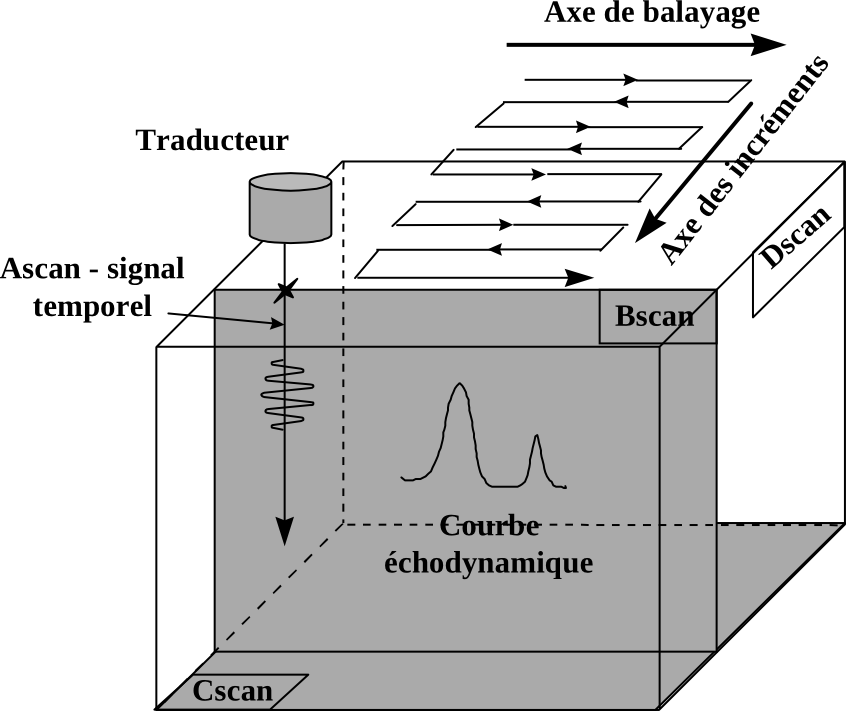
\includegraphics[scale=0.7]{img/scan.png}
%	\caption{\label{scan} Schéma des différents modes de représentation des signaux temporels (extrait de \cite{chassignole}).}
%\end{figure} 

\begin{figure}
	\centering
	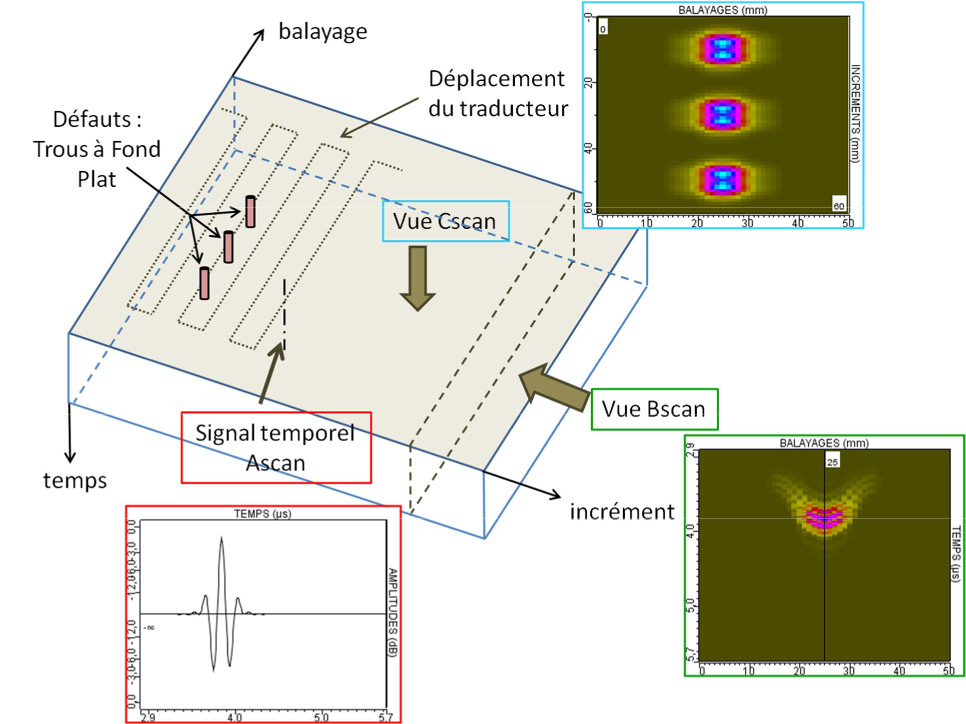
\includegraphics[scale=0.7]{img/scan2.png}
	\caption{\label{scan} Schéma des différents modes de représentation des signaux temporels (extrait de \cite{bannouf}).}
\end{figure}

En revanche, le Sscan ne peut être réalisé qu'avec des transducteurs multi-éléments. Il correspond a un ensemble de Ascans réalisés sans déplacement du transducteur mais en appliquant une loi de retard aux éléments permettant de réaliser un balayage du point focal. Le Sscan permet donc d'imager des pièces partiellement accessible, et augmente la probabilité de repérer un défaut en offrant plusieurs angles d'observation.\\

Cependant, la localisation dans la pièce des réflecteurs à l'origine des différents échos visibles sur les signaux temporels mesurés n'est possible que si la vitesse de propagation des ondes est connue. Les Bsans dits "vrais" sont des Bscans sur lesquels des corrections liées à la vitesse ou à l'angle d'incidence sont appliqués.


\section{Méthodes par retard et sommation}
Ces données temporelles peuvent aussi être post-traitées de manière à obtenir une représentation spatiale de la pièce. Si la vitesse du milieu de propagation est connue, une analyse des temps de vol des échos permet en effet d'établir une carte du milieu. \\

Il est aussi possible de sommer un ensemble de Ascans de façon cohérente, permettant ainsi de reproduire une focalisation en tous points de la zone à inspecter. C'est que proposent la méthode Synthetic Aperture Focusing Technique \citep{doctor_saft} à partir des signaux recueillis par un mono-éléments. Ce procédé est généralisé à un ensemble de capteurs et d'émetteurs dans la méthode Total Focusing Method \citep{holmes_tfm}. 

L'intensité $I$ de l'image obtenue au point de coordonnées $\bm{r}$ est alors donnée par la relation suivante : 

\begin{equation*}
	I(\bm{r})= \displaystyle\sum_{r} \displaystyle\sum_{t} s_{r,t}\left( \frac{|\bm{r} - \bm{r}_r| + |\bm{r} - \bm{r}_t|}{c}\right) \text{,}
\end{equation*}
où $\bm{r}_r$ et $\bm{r}_t$ sont les positions des récepteurs et des émetteurs, $s_{r,t}$ sont les signaux temporels pour chaque couple émetteur-récepteur et $c$ est la vitesse de l'onde dans le milieu de propagation.

Cette focalisation permet donc de couvrir l'ensemble du volume de la pièce car tous les angles peuvent être balayés, indépendamment de l'ouverture du capteur, ce qui permet une meilleure résolution que celle obtenue avec des Bscans.\\






\section{Méthodes hautes résolution}


Des méthodes de localisation de sources dites "hautes résolutions" exploitent l'ensemble des covariances des signaux temporels. Les méthodes telles que MUltiple Signal Classification \citep{schmidt} et Capon \citep{capon} proposent une décomposition en valeurs propres de cette matrice de covariance afin d'en extraire deux sous-espaces bruit et signal, diminuant ainsi la contribution énergétique du bruit. \\

La méthode de Décomposition de l'Opérateur de Retournement Temporel \citep{prada_dort} propose, de la même façon, d'interpréter l'opérateur de retournement temporel comme une matrice de covariance et de la décomposer. Cette dernière méthode est particulièrement adaptée aux milieux hétérogènes et/ou à géométrie complexe , puisqu'elle tire profit des réflexions multiples.  

Tous comme les méthode de formation de voies classiques, il est nécessaire de connaître les propriétés élastiques du milieu de propagation pour pouvoir localiser précisément les réflecteurs.\\

%(billette de titane, par exemple https://www.institut-langevin.espci.fr/IMG/pdf/jasakerbrat-2002.pdf)
%(plaque mince : ondes de lamb https://www.institut-langevin.espci.fr/IMG/pdf/JASAlamb-1998.pdf)

\section{Résolution de problème d'optimisation}

L'objectif de ces méthodes est de résoudre un problème inverse en minimisant une fonction coût traduisant l'écart entre le modèle calculé et le modèle vrai \citep{tarantola_book}. Le modèle est décrit par un nombre fini de paramètres $\bm{m}$ qui sont liés à des observables $\bm{d}_{obs}$ par l'intermédiaire de lois physiques $\bm{g}$. La résolution du problème inverse consiste donc à trouver les paramètres $\bm{m}$ optimaux à partir des données $\bm{d}_{obs}(\bm{m})$ (cf schéma de la figure~\ref{pb_inv}). 

\begin{figure}[!h]
	\centering
	\begin{tikzpicture}
		\node (param) [draw=black, align=center] at (0,0) {Paramètres initiaux \\ $\bm{m}_{0}$};
		\node (dir) [below=1cm of param , draw=black,align=center] {Problème direct \\ $\bm{g}(\bm{m})$};
		\path[->, thick,shorten <=2pt,shorten >=2pt] (param) edge (dir);
		\node (fc) [draw=black,right=2cm of dir, align=center] {Fonction de coût \\ $\text{écart}\hspace{-1mm}\left(\bm{d}_{obs}, \bm{d}_{cal}(\bm{m})\right)$};
		\path[->, thick,shorten <=2pt,shorten >=2pt] (dir) edge (fc);
		\node (m) [draw=black, below right= and -0.5cm of dir, align=center] {Problème inverse \\$\bm{m}+\Delta\bm{m}$};
		\path[->, thick,shorten <=2pt,shorten >=2pt] (fc) edge (m);
		\path[->, thick,shorten <=2pt,shorten >=2pt] (m) edge (dir);
	\end{tikzpicture} 
	\caption{\label{pb_inv} Schéma de résolution d'un problème d'optimisation.}
\end{figure}

Ces problèmes sont, en général, non-linéaires, car les observables ne dépendent pas linéairement des paramètres du modèle. De plus, si le nombre de paramètres est grand devant le nombre d'observables, ils sont également mal posés.\\

\subsection{Résolution du problème direct}

Le problème direct peut être résolu soit par des méthodes analytiques (représentation intégrale, méthodes modales,\ldots) soit par des méthodes numériques. Parmi les méthodes numériques les plus usitées figurent : les méthodes de différences finies (\citealp{virieux_86}, à l'ordre 2 et \citealp{levander}, à l'ordre 4), les méthodes des éléments finis (Galerkin discontinu par exemple : \citealp{brossier_these}) ou volumes finis \citep{brossier_2008}, les lancers de rayons \citep{virieux_ray}. 

\subsection{Résolution du problème inverse}
Si le problème direct possède une solution unique, ce n'est pas le cas du problème inverse.
Lorsque le nombre de paramètres est grand, le problème inverse ne peut pas être résolu par une recherche exhaustive dans l'espace des solutions. La recherche de solution peut donc se faire de manière semi-globale ou locale.\\

\subsubsection{Les méthodes semi-globales}
Les méthodes semi-globales consiste a parcourir l'espace des solutions avec une approche statistiques. Les plus connues sont les améliorations de celle de Monte Carlo comme le recuit simulé \citep{tarantola_book, sen} ou  la méthode de Monte-Carlo par chaînes de Markov \citep{zhang}, ainsi que les algorithmes génétiques. Elles permettent d'assurer une convergence avec peu d'\emph{a priori} sur le modèle initial.\\

\subsubsection{Les méthodes locales}
Lorsque que le modèle initial comporte suffisamment d'informations pour que le problème se situe proche du minimum global recherché, des méthodes d'optimisation moins coûteuses sont envisageables. Ces méthodes se basent sur l'estimation du gradient et du hessien de la fonction coût pour estimer sa plus forte pente et sa courbure.\\

La méthode de recherche linéaire la plus simple est celle du gradient (ou algorithme de la plus forte pente), qui permet d'effectuer au point courant, un pas de descente dans la direction opposée au gradient. Les directions de descentes successives sont alors orthogonales, ce qui ne permet pas une convergence très rapide. \\
La méthode du gradient conjugué propose de combiner les directions de descente des itérations précédentes de façon à accélérer la convergence. Cette méthode populaire est celle utilisée par Mora et Tarantola dans les années 80 \citep{tarantola_84, mora_87a, mora_87b}. Le hessien n'est pas calculé, mais cette méthode nécessite le calcul de deux problèmes directs supplémentaires. \\

Les méthodes full-Newton et Gauss-Newton utilisent le calcul du hessien (complet pour la première, approximé pour la seconde), ce qui permet une convergence plus rapide qu'avec la méthode du gradient conjugué, sans coût excessif supplémentaire \citep{pratt_98}.\\

Enfin, le hessien peut également être estimé à partir des gradients des itérations précédentes, par la méthode quasi-Newton \citep{nocedal}, avec l'algorithme BFGS (Broyden, Fletcher, Goldfarb, Shanno), par exemple. Cet algorithme ayant un gros coût de stockage, il existe des versions allégées fournissant une estimation du hessien à partir du stockage de quelques itérations seulement (L-BFGS). 
\subsection{Cartographie ou contour}
Comme le souligne les auteurs du chapitre 1.4 de BruneauPotel, le problème inverse peut être résolu suivant deux approches : 
\begin{itemize}
	\item un formalisme en intégrales de contour où les paramètres reconstruits sont ceux décrivant ces contours. Cela revient donc à déterminer la topologie d'un milieu. Le gradient, donné par la dérivée de la fonction coût par rapport à la topologie, indique donc directement la position d'un défaut à fort contraste. \cite{dominguez} et \cite{rodriguez} utilisent par exemple cette approche pour des applications en contrôle non destructif. Cette approche permet par exemple d'imager des défauts liés à une absence de matière (porosité, fissure, délaminage,\ldots) mais ne permet pas de caractériser des défauts de contraste plus faible (inclusion, corps étranger,\ldots).
	\item une reconstruction pixelisées d'un ensemble de paramètres. C'est l'approche adoptée pour la FWI et qui est décrite au chapitre~\ref{fwi}.
\end{itemize}


%-mais aussi : diffraction tomograhy, filtered backpropagation... : techniques basées sur une version linéarisée des équations, born approx par ex, kirchhoff approx


\section{Spécificités de l'imagerie de soudure}

Nombre de ces méthodes sont peu adaptées à l'imagerie de soudure. En effet, comme le montrent les macrographies de la figure~\ref{soudure}, les passes multiples et la cristallisation inhomogène rendent la soudure fortement anisotrope \citep{chassignole}. Cette anisotropie varie d'unes soudure à une autre puisqu'elle dépend des paramètres de soudage. En conséquence, cette anisotropie engendre une courbure voire une division du faisceau ultrasonore. Les scans sont alors difficiles à analyser (cf figure \ref{echos}), les méthodes par retard et sommation ne permettent pas de relocaliser précisément un réflecteur et les images obtenues sont très sujettes aux artefacts provenant d'échos mal interprétés.

\begin{figure}[!h]
	\hspace{-2cm}
    \centering
    \begin{subfigure}[c]{0.25\textwidth}
    	\centering
        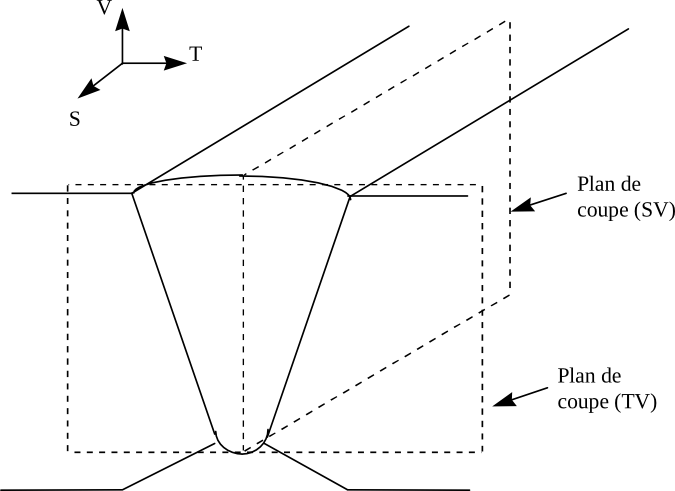
\includegraphics[height=3.5cm]{./img/soudure3.png}
        \vspace{0.03cm}
        \caption{\centering  Définition des plans de coupe.}
    \end{subfigure}
    \hspace{1cm}
    \begin{subfigure}[c]{0.25\textwidth}
    	\centering
        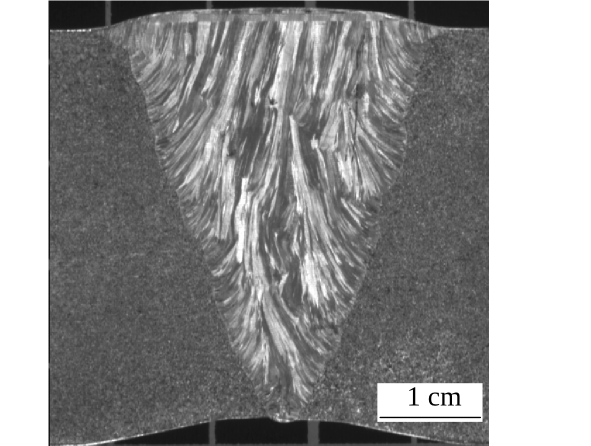
\includegraphics[height=4cm]{./img/soudure1.png}
        \caption{\centering  Coupe dans le plan (TV).}
    \end{subfigure}
        \hspace{1.5cm}
    \begin{subfigure}[c]{0.25\textwidth}
    	\centering
		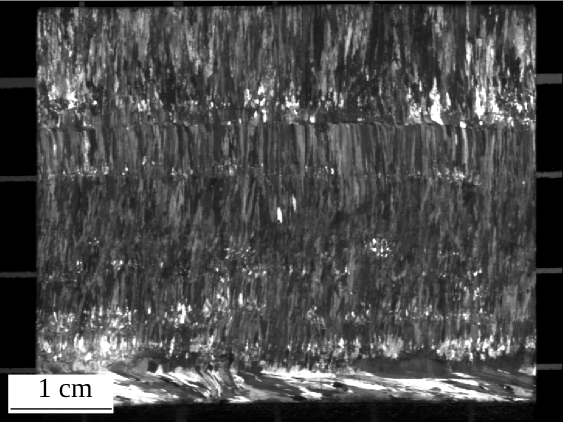
\includegraphics[height=4cm]{./img/soudure2.png}
        \caption{\centering Coupe dans le plan (SV).}
    \end{subfigure}
    \caption{Macrographie d'une soudure industrielle en acier inoxydable en acier austénitique \citep{chassignole}. À gauche : coupe dans le plan $(x,z)$, à droite : coupe dans le plan $(x,y)$.\label{soudure}}
\end{figure}

\begin{figure}[!h]
    \centering
    \begin{subfigure}[c]{0.3\textwidth}
    	\centering
        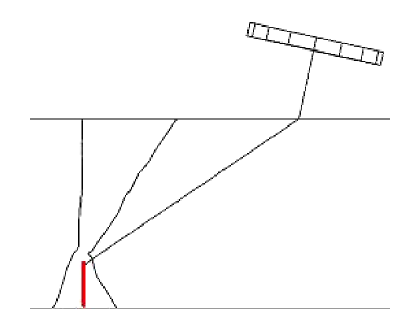
\includegraphics[height=4cm]{img/chassignole_echos_config.png}
        \caption{Configuration de mesure. En rouge : encoche de 15~mm de haut dans la soudure.}
    \end{subfigure}
    \hspace{1cm}
    \begin{subfigure}[c]{0.3\textwidth}
    	\centering
        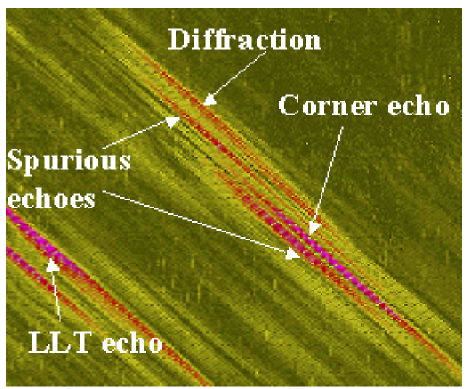
\includegraphics[height=4cm]{img/chassignole_echos.png}
        \caption{Bscan}
    \end{subfigure}
    \caption{Illustration de la perturbation du faisceau ultrasonore dans une sourdure. Images extraites de \cite{chassignole_beam}. LLT echo : Réflexion de l'onde longitudinale (L) sur le bord de soudure puis réflexion de cette onde L sur l'encoche avec conversion en mode transverse (T).  }\label{echos}
\end{figure}

De manière générale, les méthodes nécessitant une bonne connaissance du matériau ne sont pas adaptées à l'imagerie de soudure ; tenter de reconstruire les paramètres élastiques de la soudure par une résolution de problème inverse semble être une approche plus appropriée.




\todo[inline]{}

%hohne\_2012 pour images SAFT


%gardahaut pour porpagation de rai CIVA

%Born : linéarise le pb ? (pour faible contraste, adapté au cnd ?) brossier these dit que c'est pas linéarisé et qu'on a donc le champ d'onde complet

%+acoustique non-linéaire : Nonlinear signal processing for ultrasonic imaging of material complexity (dos santos) par ex


\chapter{L'inversion de formes d'onde \label{fwi}}

L'inversion de forme d'ondes (ou FWI, pour \emph{Full Waveform Inversion}) est une méthode quantitative d'imagerie développée dans un contexte géophysique permettant de reconstruire des paramètres élastiques par résolution d'un problème inverse posé dans les années 80 par \cite{lailly} et \cite{tarantola_84}. Par opposition à des inversions du type tomographie qui n'utilisent que partiellement les informations contenues dans les champs mesurés, l'inversion de formes d'onde utilise l'ensemble des données sans hypothèses. \\

Le principe général est de calculer des données $\bm{d}_{cal}$ issues d'un modèle (résolution du problème direct)  puis de minimiser l'écart entre ces données et les données réelles $\bm{d}_{obs}$ issues de la mesure en modifiant les paramètres du modèle \citep{virieux_review}. Cette démarche est résumée en figure~\ref{schema_fwi} et l'ensemble des étapes est détaillé par la suite.


\begin{figure}[!h]
	\begin{tikzpicture}
		\node (init) [draw=black, align=center] at (0,0) {Paramètres initiaux \\ $\bm{m}_{0}$};
		\node (dir) [below=1cm of init , draw=black,align=center] {Problème direct :\\ éléments finis ou différences finies};
		\path[->, thick,shorten <=2pt,shorten >=2pt] (init) edge (dir);
		\node (fc) [draw=black,right=2cm of dir, align=center] {Fonction de coût \\ $C(\bm{m})=\frac{1}{2}||\bm{d}_{obs}-\bm{d}_{cal}(\bm{m})||^{2}$};
		\path[->, thick,shorten <=2pt,shorten >=2pt] (dir) edge (fc);
		\node (m) [draw=black, below right= and -5.5cm of dir, align=center] {Problème inverse : \\~\\ 
			\begin{minipage}{0.3\textwidth}
				\centering
				Calcul du gradient $C'(\bm{m})$
				Calcul du hessien $C''(\bm{m})$
			\end{minipage}
			\vline
			\begin{minipage}{0.2\textwidth}
				\centering
				~$\bm{\Delta m}=-C''C'$
			\end{minipage}
			\vline
			\begin{minipage}{0.3\textwidth}
				\centering
				Mise à jour du modèle : \\ $\bm{m} := \bm{m}+ \bm{\Delta m}$
			\end{minipage}
		};
		\path[->, thick,shorten <=2pt,shorten >=2pt] (fc) edge (m);
		\path[->, thick,shorten <=2pt,shorten >=2pt] (m) edge (dir);		
	\end{tikzpicture} 
	\caption{Schéma du principe de la FWI.\label{schema_fwi}}
\end{figure}

%"inversion approach resembles prestack, reverse-time mi-
%gration but differs in that the problem is formulated in
%terms of velocity (not reflectivity), and the method is
%fully iterative."PRATT99

%rodirguez 2014 : Full waveform
%inversion should not to be mistaken for migration techniques that
%are based on Claerbout’s ‘‘imaging principle’’ : J.F. Claerbout, Toward a unified theory of reflector mapping, Geophysics 36 (3)
%(1971) 467–481.which defines a
%reflectivity field by the ratio of upgoing and downgoing wave
%fields. Neverthelesss

\section{Problème direct \label{pd_dir}}

Dans le cas de l'imagerie par ultrason, résoudre le problème direct revient à trouver la solution de l'équation d'onde linéarisée. Il est fréquent que l'hypothèse d'une propagation acoustique soit faite en prospection géophysique. Cette approximation a pour but de réduire fortement le coût des calculs et est justifiée par le fait que la trace des ondes de compression soit dominante dans les données de mesures. De plus, en réduisant le nombre de paramètres du modèle, le problème est rendu moins non-linéaire. Cependant, cette approximation ne permet pas une caractérisation complète du milieu et, pour une application en CND, demande un pré-traitement parcimonieux des données et retire notamment la précision qu'offrent les ondes de cisaillement par leur faible longueur d'onde.\\~\\




 Pour résoudre l'équation d'onde, parmi les approches qui nécessitent de faire le moins d'hypothèse sur le champ d'onde et sur le milieu de propagation figurent les différences finies et les éléments finis. Les différences finies sont les plus faciles à développer et à implémenter. Elles permettent de discrétiser les dérivées temporelles et spatiales par des différences d'ordre 2 \citep{virieux_86} ou d'ordre 4 \citep{levander}. Cependant, contrairement aux éléments finis, elles imposent l'utilisation de grilles régulières et ne permettent donc pas d'adapter localement le pas de grille à la géométrie ou à la complexité du milieu. \\ Les éléments finis se prêtent mieux aux maillages non-structurés. Leur solution est développée sur des basent de fonction (d'ordre élevé pour les éléments finis spectraux) et permettent de prendre simplement en compte les conditions limites.\\
 
Deux types de conditions limites sont nécessaires pour le modèle de soudure à 2 dimensions (2D) : une condition parfaitement réfléchissante (Dirichlet) au niveau des surfaces de la plaque (en considérant une mesure dans l'air, le couplage fluide structure est négligeable) et une condition absorbante pour représenter la plaque loin de la zone d'étude (cf figure~\ref{BC}). Les conditions absorbantes sont modélisées à l'aide de \emph{Perfectly Matched Layers} (PML) qui simulent une forte atténuation dans une zone restreinte de manière anisotrope (seule la composante normale de l'onde est atténuée).

\begin{figure}[!h]
	\centering
	\begin{tikzpicture}
		\draw (0,0) -- (9,0) ;
		\draw (0,-2) -- (9,-2) ;
		\filldraw [fill=gray, fill opacity=0.5, draw=none] (3.5,0) -- (4.5,-2) -- (5.5,0)  ;
		\node (centre) at (4.3,-1) {};
		\node (soudure) at (7,-2.5) {soudure};
		\draw[<-,thick] (centre) -- (soudure);
		\node (fs) [align=left] at (2.5,0.3) {Condition de Dirichlet}	;
		\node (fs2)[align=left] at (2.5,-2.3) {Condition de Dirichlet};
		\draw[dotted] (0,0) -- (0,-2);
		\draw[dotted] (9,0) -- (9,-2);
		\node (g) [align=center] at (-1.3,-1) {Conditions \\ absorbantes \\ (PML)};
		\node (d) [align=center] at (10.3	,-1	) {Conditions \\ absorbantes \\ (PML)};
		\draw[dashed] (0,0) -- (-1,0);
		\draw[dashed] (0,-2) -- (-1,-2);
		\draw[dashed] (9,0) -- (10,0);
		\draw[dashed] (9,-2) -- (10,-2);
	\end{tikzpicture}
	\caption{Représentation des deux types de conditions limites du modèle de soudure 2D.\label{BC}}
\end{figure}

\todo[inline]{Questions : qu'est-ce qui est fait en fréquence, qu'est qui est fait en temps (modèle, inversion) ?}

Le problème peut-être résolu dans le domaine temporel ou dans le domaine fréquentiel \citep{vigh_2008}. Le domaine temporel laisse la possibilité d'effectuer une sélection des arrivées d'ondes par fenêtrage temporel mais présente une plus forte susceptibilité au phénomène de saut de phase (décrit dans le paragraphe ????).  De plus, la résolution par différences finies dans le domaine temporel impose un critère de stabilité Courant-Friedrichs-Lewy (CFL) qui peut-être contraignant, surtout en 3D. Dans le domaine fréquentiel, l'équation d'onde étant réduite à un système d'équations linéaires, il est possible d'utiliser des méthodes de résolution directe du type décomposition LU bien qu'en pratique, les performances de ces méthodes soient limitées pour des problèmes comportant un grand nombre d'inconnues.  Les principaux avantages d'une résolution du problème direct dans le domaine fréquentiel sont donc d'intégrer facilement les phénomènes d'atténuation et de permettre une sélection fine des fréquences d'intérêt. \\~\\







\section{Problème inverse}

Le problème inverse est un problème d'optimisation locale visant à réduire l'écart entre les données observées $\bm{d}_{obs}$ et les données calculées $\bm{d}_{cal}(\bm{m})$ pour chaque couple source-récepteur, en ajustant le modèle constitué de M paramètres $\bm{m}$. L'idée est donc de minimiser la norme au sens des moindres carrés de la différence $\bm{d}_{obs}-\bm{d}_{cal}(\bm{m})$ définie comme suit : 
\begin{equation}
	C(\bm{m})=\frac{1}{2}||\bm{d}_{obs}-\bm{d}_{cal}(\bm{m})||^{2}\text{.}
	\label{norm}
\end{equation}
 Le minimum de cette fonction de coût est atteint lorsque la dérivée par rapport aux paramètres du modèle s'annule. Un développement de Taylor au second ordre de $C(\bm{m}+ \bm{\Delta m})$ permet d'écrire : 
 \begin{equation}
 	\frac{\dd C(\bm{m}+\bm{\Delta m})}{\dd m_{i}}= \frac{\dd C(\bm{m})}{\dd m_{i}} + \displaystyle\sum_{j}^{M} \frac{\dd^{2} C(\bm{m})}{\dd m_{j} \dd m_{i}}\Delta m_{j}\text{.}
 \end{equation}
Les termes d'ordres plus élevés sont nuls si le problème direct est linéaire. Le minimum de la fonction de coût est alors atteint en une seule itération en annulant la dérivée : 
\begin{equation}
	\frac{\dd C(\bm{m}+\bm{\Delta m})}{\dd m_{i}} = 0 ~~~~~\Leftrightarrow ~~~~~ \Delta m _{j} = -\left( \frac{\dd ^{2} C(\bm{m})}{\dd m_{j} \dd m_{i} }\right)^{-1} \frac{\dd C (\bm{m})}{\dd m_{i}} \text{.}
\end{equation}
En FWI, le problème inverse n'étant pas linéaire, cette inversion est réalisée sur plusieurs itérations.\\
La direction de descente est donc donnée par le gradient et la dérivée seconde (hessien) donne la courbure de la fonction de coût.\\



\subsection{Calcul du gradient}

D'après l'expression de la norme~\ref{norm}, sa dérivée par rapport aux paramètres $\bm{m}$ (le gradient) est donc : 
\begin{equation}
	 \frac{\dd C (\bm{m})}{\dd m_{i}} = -\tr{\left( \frac{\dd \bm{d}_{cal}(\bm{m}) }{\dd m_{i}} \right)} ( \bm{d}_{obs} - \bm{d}_{cal}(\bm{m})) \text{.}
	 \label{eq_grad}
\end{equation}\\



Le problème direct décrit au paragraphe précédent~(\ref{pd_dir}) peut se mettre sous la forme :
\begin{equation}
	\bm{A}(\bm{m},\bm{r},\xi)\bm{d}_{cal}(\bm{m},\bm{r},\xi)=\bm{s}(\bm{r},\xi)\text{,}
	\label{eq_pb_dir}
\end{equation}

où $\bm{r}$ est la variable d'espace et $\xi$ est le temps ou la fréquence. $\bm{A}$ est un opérateur correspondant à l'équation d'onde et $\bm{s}$ est le terme source. Notons que le vecteur de données $\bm{d}_{cal}$ a une longueur égale au nombre de récepteur et doit donc être étendu de façon a avoir la même longueur que l'espace du problème direct. La dérivée de l'équation~\ref{eq_pb_dir} par rapport à $\bm{m}$ s'écrit : 
\begin{equation}
	\bm{A} \frac{\dd \bm{d}_{cal}(\bm{m})}{\dd m_{i}} + \frac{\dd A}{\dd m_{i}}\bm{d}_{cal}(\bm{m}) = \bm{0} \text{.}
\end{equation}

On a donc : 
\begin{equation}
	\tr{\left( \frac{\dd \bm{d}_{cal}(\bm{m})}{\dd \bm{m}}  \right)} = - \tr{\bm{d}_{cal}(\bm{m})} \tr{\left( \frac{\dd \bm{A}}{\dd \bm{m}} \right)} \tr{A^{-1}}
	\label{sub}
\end{equation} 	

Finalement, en reportant cette expression dans l'équation~\ref{eq_grad}, on obtient l'expression du gradient : 
\begin{equation}
	 \frac{\dd C (\bm{m})}{\dd m_{i}} = \tr{\bm{d}_{cal}(\bm{m})}  \tr{\left( \frac{\dd \bm{A}}{\dd m_{i}}\right)} \tr{\bm{A}} (\bm{d}_{obs} - \bm{d}_{cal}(\bm{m}))^* = \tr{\bm{d}_{cal}(\bm{m})} \tr{\left( \frac{\dd \bm{A}}{\dd m_{i}}\right)} \lambda^*
\end{equation}
\todo[inline]{conjugué de $\Delta d $ ?}

Le champ $\lambda^*$ correspond donc à la rétropopagation des résidus $( \bm{d}_{obs} - \bm{d}_{cal}(\bm{m}))^*$. L'opérateur conjugué $^*$ indique une propagation en temps inverse, ce qui permet, comme en retournement temporel \citep{prada_2002}, une focalisation sur les éléments diffractant absents du modèle initial. Cette expression du gradient peut également être obtenu par le formalise de l'état adjoint \citep{plessix}.\\
\todo[inline]{quid de dA/dm ? Diagramme de rayonnement ?}

La substitution~\ref{sub} permet d'éviter le calcul de la matrice de sensibilité $\tr{\left( \frac{\dd \bm{d}_{cal}(\bm{m}) }{\dd m_{i}} \right)}$ . Le calcul du gradient découle donc du calcul de deux problèmes directs : 
\begin{equation*}
	\bm{A}(\bm{m})\bm{d}_{cal}(\bm{m})=\bm{s} ~~~~~~~\text{et}~~~~~~~\bm{A}(\bm{m}) \lambda^*(\bm{m})=( \bm{d}_{obs} - \bm{d}_{cal}(\bm{m}))^*
\end{equation*}

\subsection{Calcul du hessien}

La méthode d'optimisation choisie pour la FWI est une méthode quasi-Newton qui propose d'utiliser une version approximée de l'inverse du hessien, calculée à partir de valeurs précédentes du gradient.  \cite{brossier_2009} montrent que cette méthode, développée avec l'algorithme L-BFGS, est plus performante que la méthode du gradient conjugué préconditionné en terme de convergence. 

\subsection{Régularisation}

Le problème étant mal-posé, il est nécessaire de limiter les artefacts haute-fréquences venant perturber $\bm{\Delta m}$. Pour cela, il est possible d'ajouter un terme de pondération à la fonction de coût qui permet de lisser le modèle. Ce lissage peut aussi être directement appliqué à $\bm{\Delta m}$ sous forme de filtre spatial adapté à la longueur d'onde correspondant à la fréquence d'inversion.

\section{Problématiques liées à l'inversion}

\subsection{Choix du modèle initial}
Afin d'assurer une convergence vers le minimum global, il est nécessaire que le modèle initial se situe dans le bassin d'attraction de la fonctionnelle. Pour cela, il faut s'assurer que le modèle soit cinématiquement acceptable en levant l’ambiguïté sur la phase. Les données temporelles issues de ce modèle doivent donc avoir un retard de moins d'une demi-longueur d'onde par rapport aux données observées vraies. Si cette condition n'est pas respectée, l'algorithme ne permettra pas un bon réajustement des phases et convergera vers un minimum local (cf~\ref{ambig_phase}).

\begin{figure}[!h]
	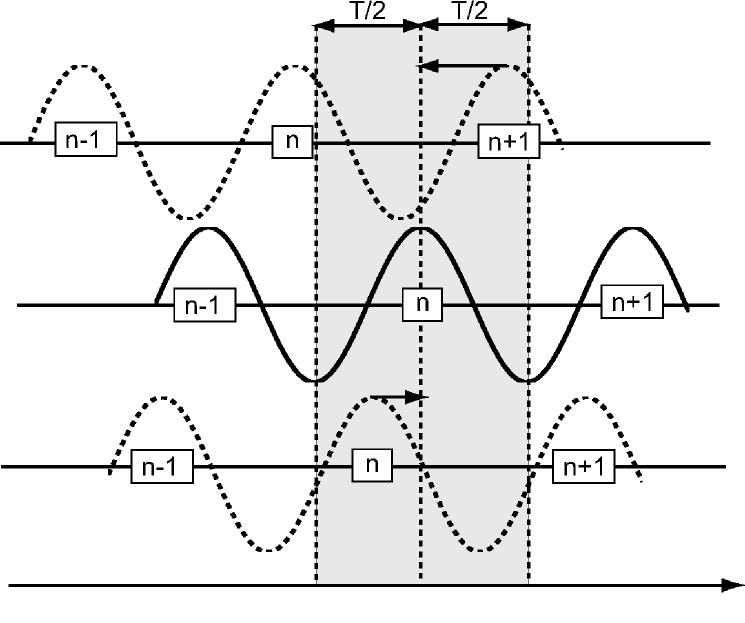
\includegraphics[scale=0.8]{img/ambig_phase.png}
	\caption{Illustration de l'ambiguïté sur la phase (extraite de \cite{brossier_these}). En haut, le déphasage est supérieur à $T/2$, les arches sont mal ajustées. En bas, le déphasage est inférieur à $T/2$, les phases sont bien ajustées. \label{ambig_phase}}
\end{figure}

 Dans cette étude, 

À défaut de disposer à un modèle initial cinématiquement acceptable, il est possible de d'appliquer un ensemble de stratégies permettant de limiter ces artefacts : introduire progressivement les sources ou récepteurs les plus éloignés, rallonger progressivement les temps d'acquisition, et inverser prioritairement les données basses fréquences.


En sismologie, une image issue de tomographie peut fournir un modèle initial assez précis. Dans cette étude, on considère que peu d'informations sont connues sur les paramètres élastiques de la soudure et le modèle initial choisi est uniforme (cf chapitre~\ref{applications}). Cependant, il serait intéressant d'envisager l'utilisation d'un modèle initial construit statistiquement à partir des résultats d'inversion d'un grand nombre de soudure.

\subsection{Inversion multi-paramètres}

Chaque changement de variable donne une nouvelle expression des différentielles des paramètres. 

choix des paramètres à inverser : ils ont différentes amplitudes et différents effets sur le champ d'onde, 
diagramme de rayonnement
citer forgues p.156 \citep{forgues}

\begin{figure}[!h]
	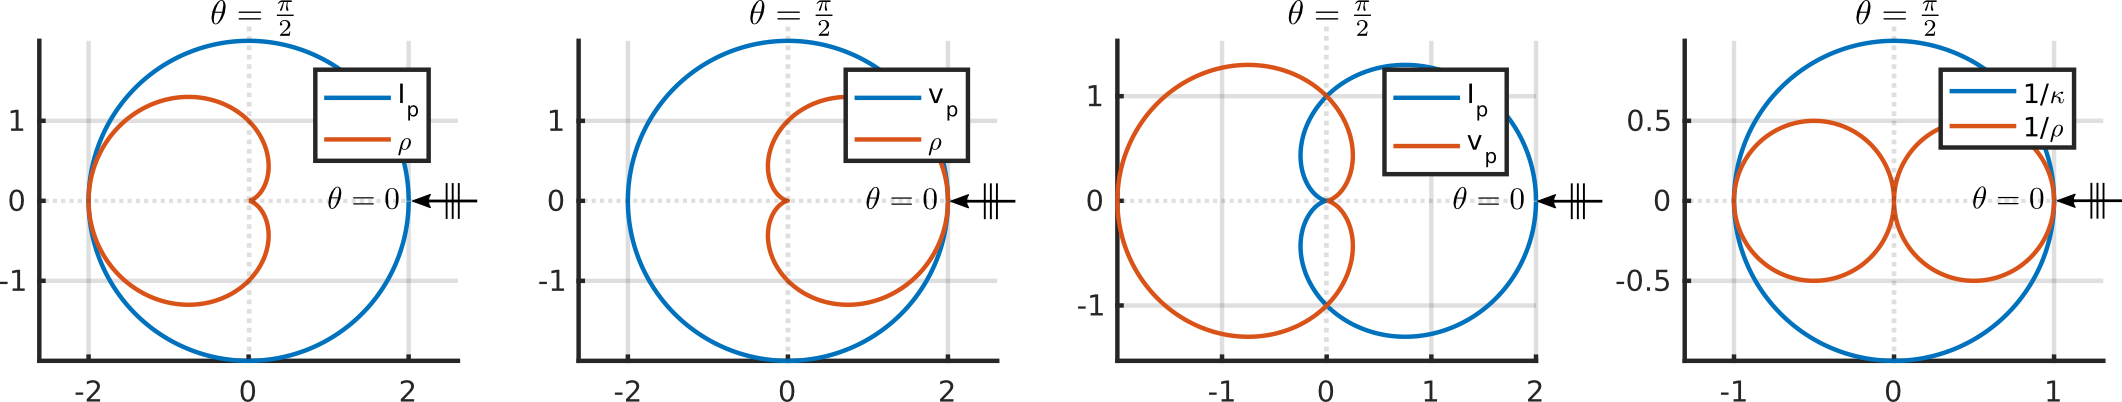
\includegraphics[scale=0.5]{img/rayonnement.png}
	\caption{Diagrammes de rayonnement pour différentes paramétrisations d'un milieu acoustique.\label{rayonnement}}
\end{figure}


\subsection{estimation de la source}






\section{resultats en geophy}

...et aussi appliqué en médical et à des ondes électromagnétiques, rayon X : natterer ?

\section{application au cnd de soudure : les problématiques}

-guide d'onde
-acquisition en surface seulement, et problématique de la soudure bombée
-anisotropie (cf image soudure) forte, qui touche not. les ondes S.
-acquisition horizontale pas idéale pour inverser la vitesse horizontale (car petits offsets et peu de courbure de rayon comme en géophys) (discuter le choix des paramètres à inverser compte-tenu de la configuration)
-sources et récepteurs mobiles 
-geophysique, dispositif de surface, donc on ne considère que les diffractions rayonnant vers la surface (soit angle de diffraction de max 180°)(Forgues, pages 160). En CND, on illumine des deux côté


%\begin{figure}
%	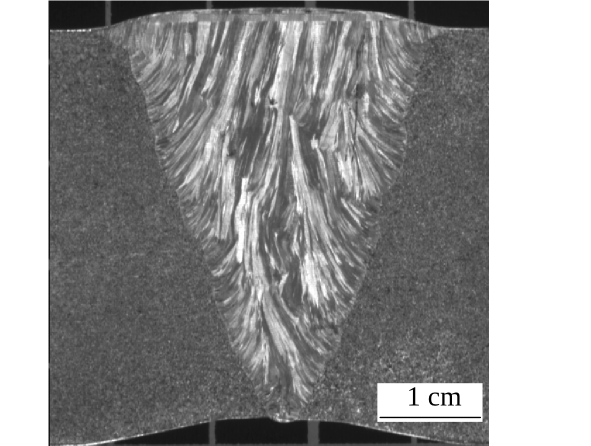
\includegraphics[height=5cm]{./img/soudure1.png}
%	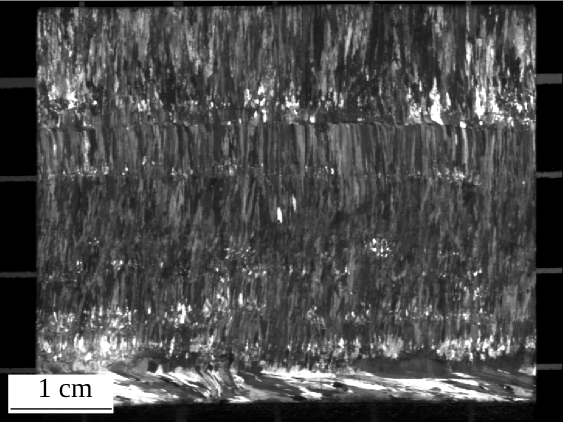
\includegraphics[height=5cm]{./img/soudure2.png}
%	\caption{Macrographie d'une soudure industrielle en acier inoxydable en acier austénitique \citep{chassignole}. À gauche : coupe dans le plan $(x,z)$, à droite : coupe dans le plan $(x,y)$.}
%\end{figure}

grains colonnaires

p91 potel bruneau : données "d'aspect limité" : il n'es tpas possible de tourner autour de l'obstace. On colpense la perte d'info en réalisant les mesures sur plusieurs freq et possibilité de déplacer capteur.




\subsection{sensibilité au bruit ?}

\todo[inline]{Les impasses volontairement faites : \\
	- détail de la discrétisation différences finies / détail des calculs FEM\\	
}


\todo[inline]{born approx}


%\chapter{Application de la FWI à des données simulées \label{applications}}

p91 potel bruneau en francais: données "d'aspect limité" : il n'est pas possible de tourner autour de l'obstacle. On compense la perte d'info en réalisant les mesures sur plusieurs freq et possibilité de déplacer capteur.

\section{Génération des données observées}

Les données de référence sont générées par la résolution d'un problème direct.
Le signal d'excitation choisi est une fonction de Ricker qui correspond à la dérivée seconde d'une Gaussienne et qui est définie de la manière suivante : 
\begin{equation}
	s(t)=(1-(t-t_{0}f\pi))^2e^{-((t-t_{0})\pi f)^2}\text{.}
\end{equation}
\todo[inline]{Est-ce réaliste ?}

Deux barrettes de 64 éléments sont utilisées en réception et en transmission. La fréquence centrale d'excitation est 2 MHz.



%\section{Discrétisation}

%Les discrétisations spatiales et temporelles sont contraintes par
%2 conditions sur la discrétisation : 
%CFL et ..points par longueur d'onde pour les schéma d'ordre ... et... (en différences finies)

\section{Analyse de résolution spatiale}
En théorie, si l'éclairage est parfait, on est limité en résolution par lambda/2 (cf review virieux ou thèse de romain : "pouvoir de résolution du gradient"). En pratique, tout comme en ray-tomo (cf wiliamson cité dans review virieux), on est très limité par l'éclairage.

Afin de déterminer le pouvoir de résolution du gradient, \cite{sirgue} réalise une analyse en onde plane comme suit. Considérons une onde plane incidente se propageant vers un point diffractant (suivant $\bm{s}$), donnant naissance en ce point à une autre onde plane se propageant suivant $\bm{r}$ (cf figure~\ref{}).\todo[inline]{pourquoi pas vers le récep ? i e Sirgue 2004 p.3 : pourquoi tous ces conjugués ?}

\begin{equation}
	k= \frac{\omega}{c} 2 \cos\left( \frac{\theta}{2}\right)
\end{equation}

La résolution est donc maximale quand $\theta=0$ et elle est alors de $\lambda/2$. La résolution s'améliore en hautes fréquences et pour des petits angles de diffraction. La géométrie du système d'acquisition a donc un impact direct sur la résolution spatiale. De plus, les surfaces libres simulent la présence de sources miroirs, d'autant plus nombreuses que le nombre de réflexions dans le guide est important. \\


supposés sans interaction

Une illustration du lien entre la couverture en nombres d'onde du milieu et l'acquisition ainsi que les sources miroirs est réalisée ci-après. Pour différentes configurations, des transformée de Fourier spatiales du gradient sont réalisées au niveau de dix-huit points diffractant, le paramètre du modèle étant la vitesse verticale (cf figure~\ref{app:config_reso}).

\begin{figure}
	\centering
	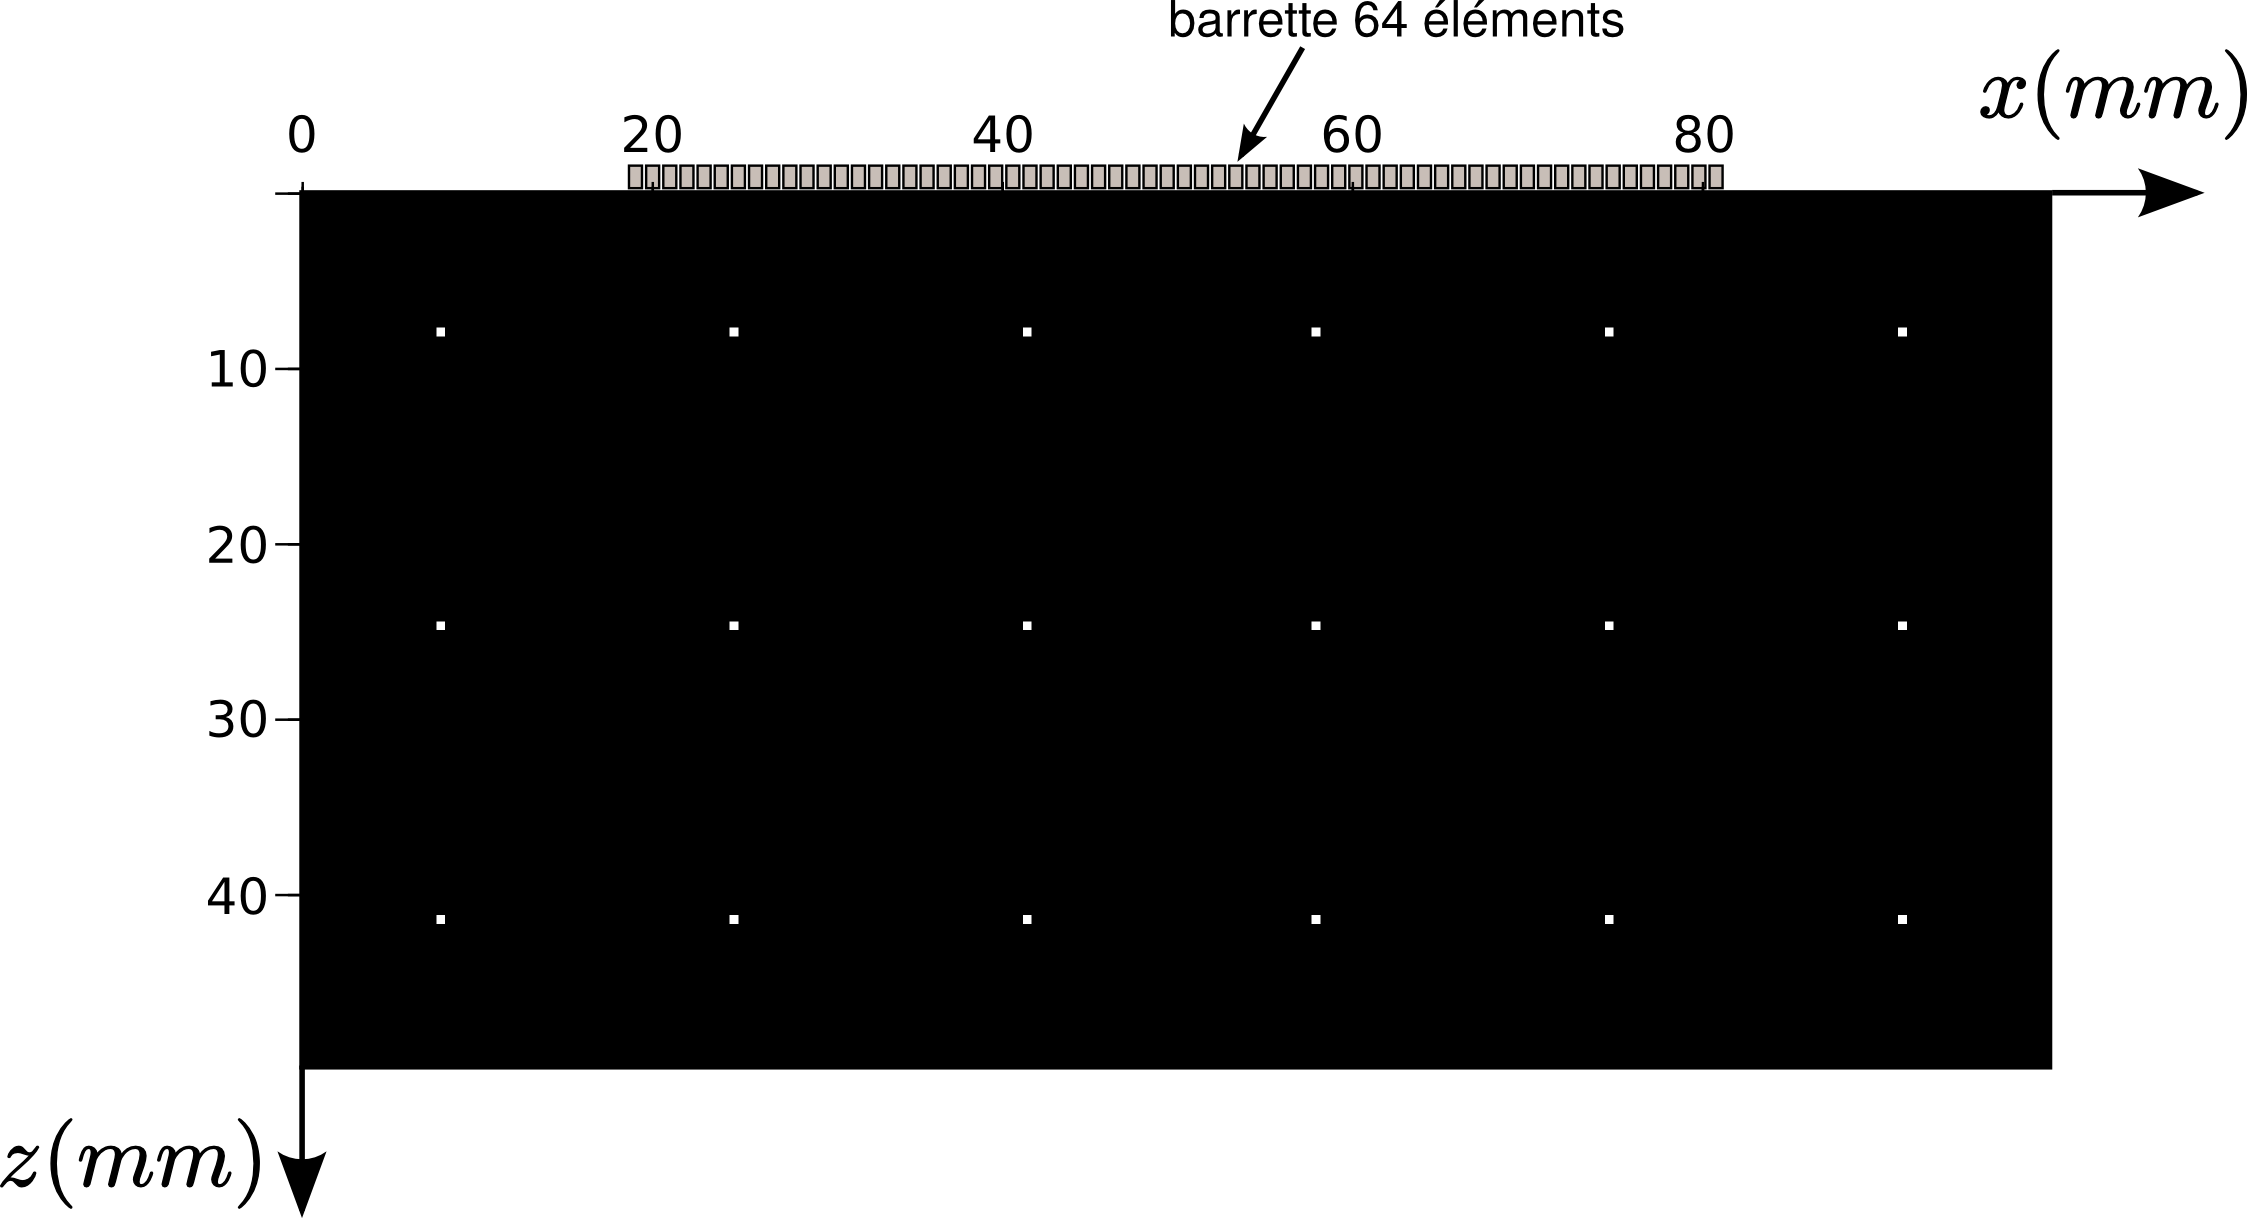
\includegraphics[height=5cm]{img/vp_scat.png}
	\caption{Configuration pour l'étude de résolution. La vitesse dans les inclusions est de 3000 m/s et de 6000 m/s ailleurs. \label{app:config_reso}}
\end{figure}

Le gradient est calculé en présence des dix-huit inclusions, sous l'hypothèse pour chaque inclusion, que la présence des autres n'intervient pas.\todo[inline]{à reformuler}

\subsection{Influence de la fréquence d'excitation}

Dans un premier temps, le milieu est entouré de conditions absorbantes. Les figures~\ref{app:150k} et~\ref{app:2M} montre la couverture en nombre d'onde obtenue dans une configuration avec une barrette excitatrice et pour deux gammes de fréquence différentes. 
    
\begin{figure}[!h]
    \centering
    \begin{subfigure}[b]{0.05\textwidth}
 		\hspace{-2cm}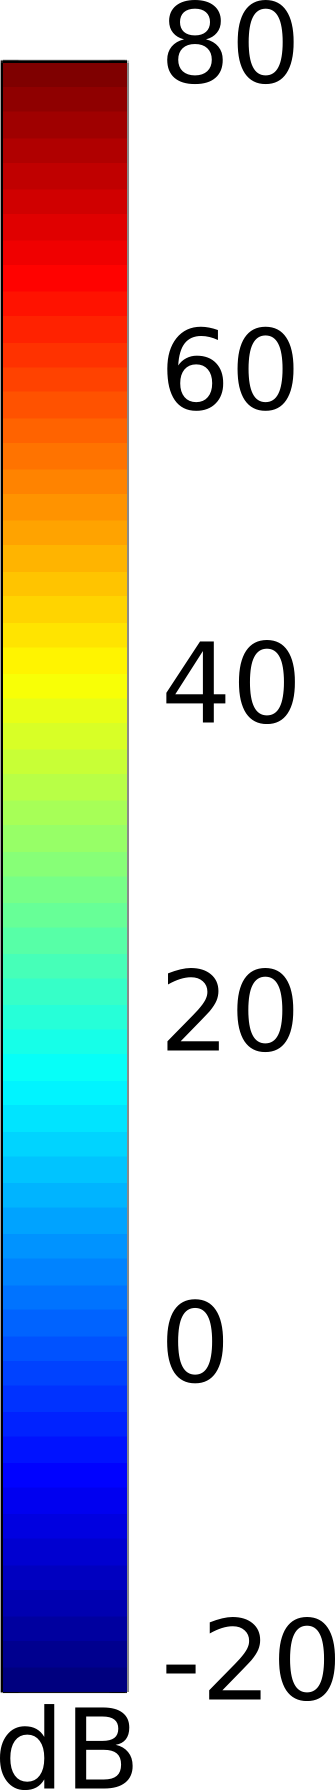
\includegraphics[width=0.5cm]{img/echelle_fft.png}\vspace{2.1cm}
	\end{subfigure}
    \begin{subfigure}[b]{0.4\textwidth}
		\hspace{-3cm}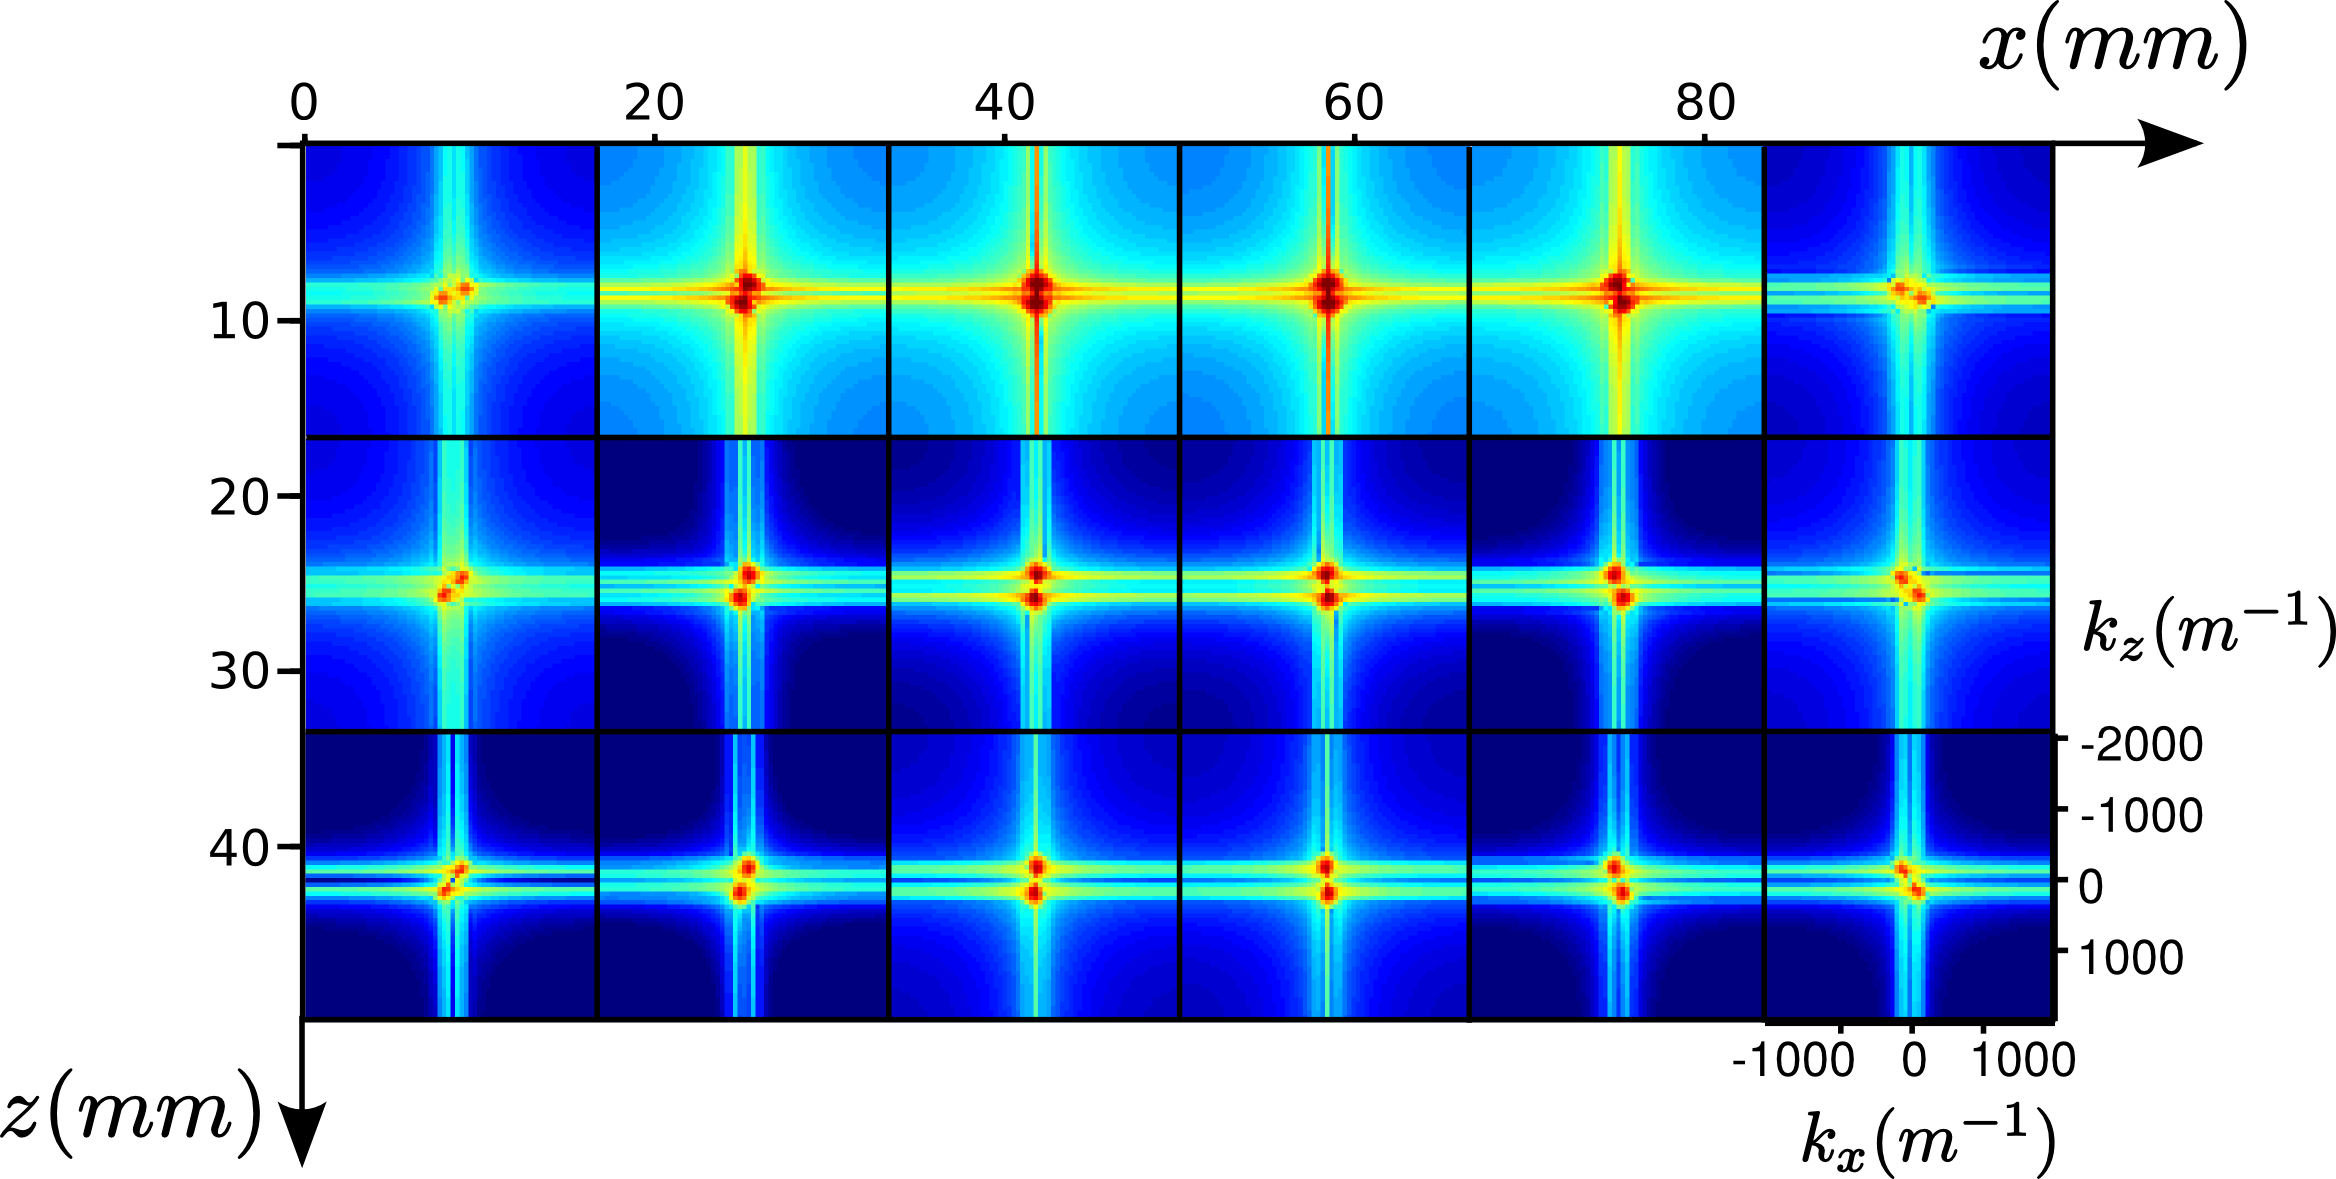
\includegraphics[width=1.5\textwidth]{img/ssfreesurf_150k}
		\caption{Excitation centrée à 150 kHz.}
		\label{app:150k}
	\end{subfigure}	
	%\hspace{0.7cm}
	\begin{subfigure}[b]{0.4\textwidth}
		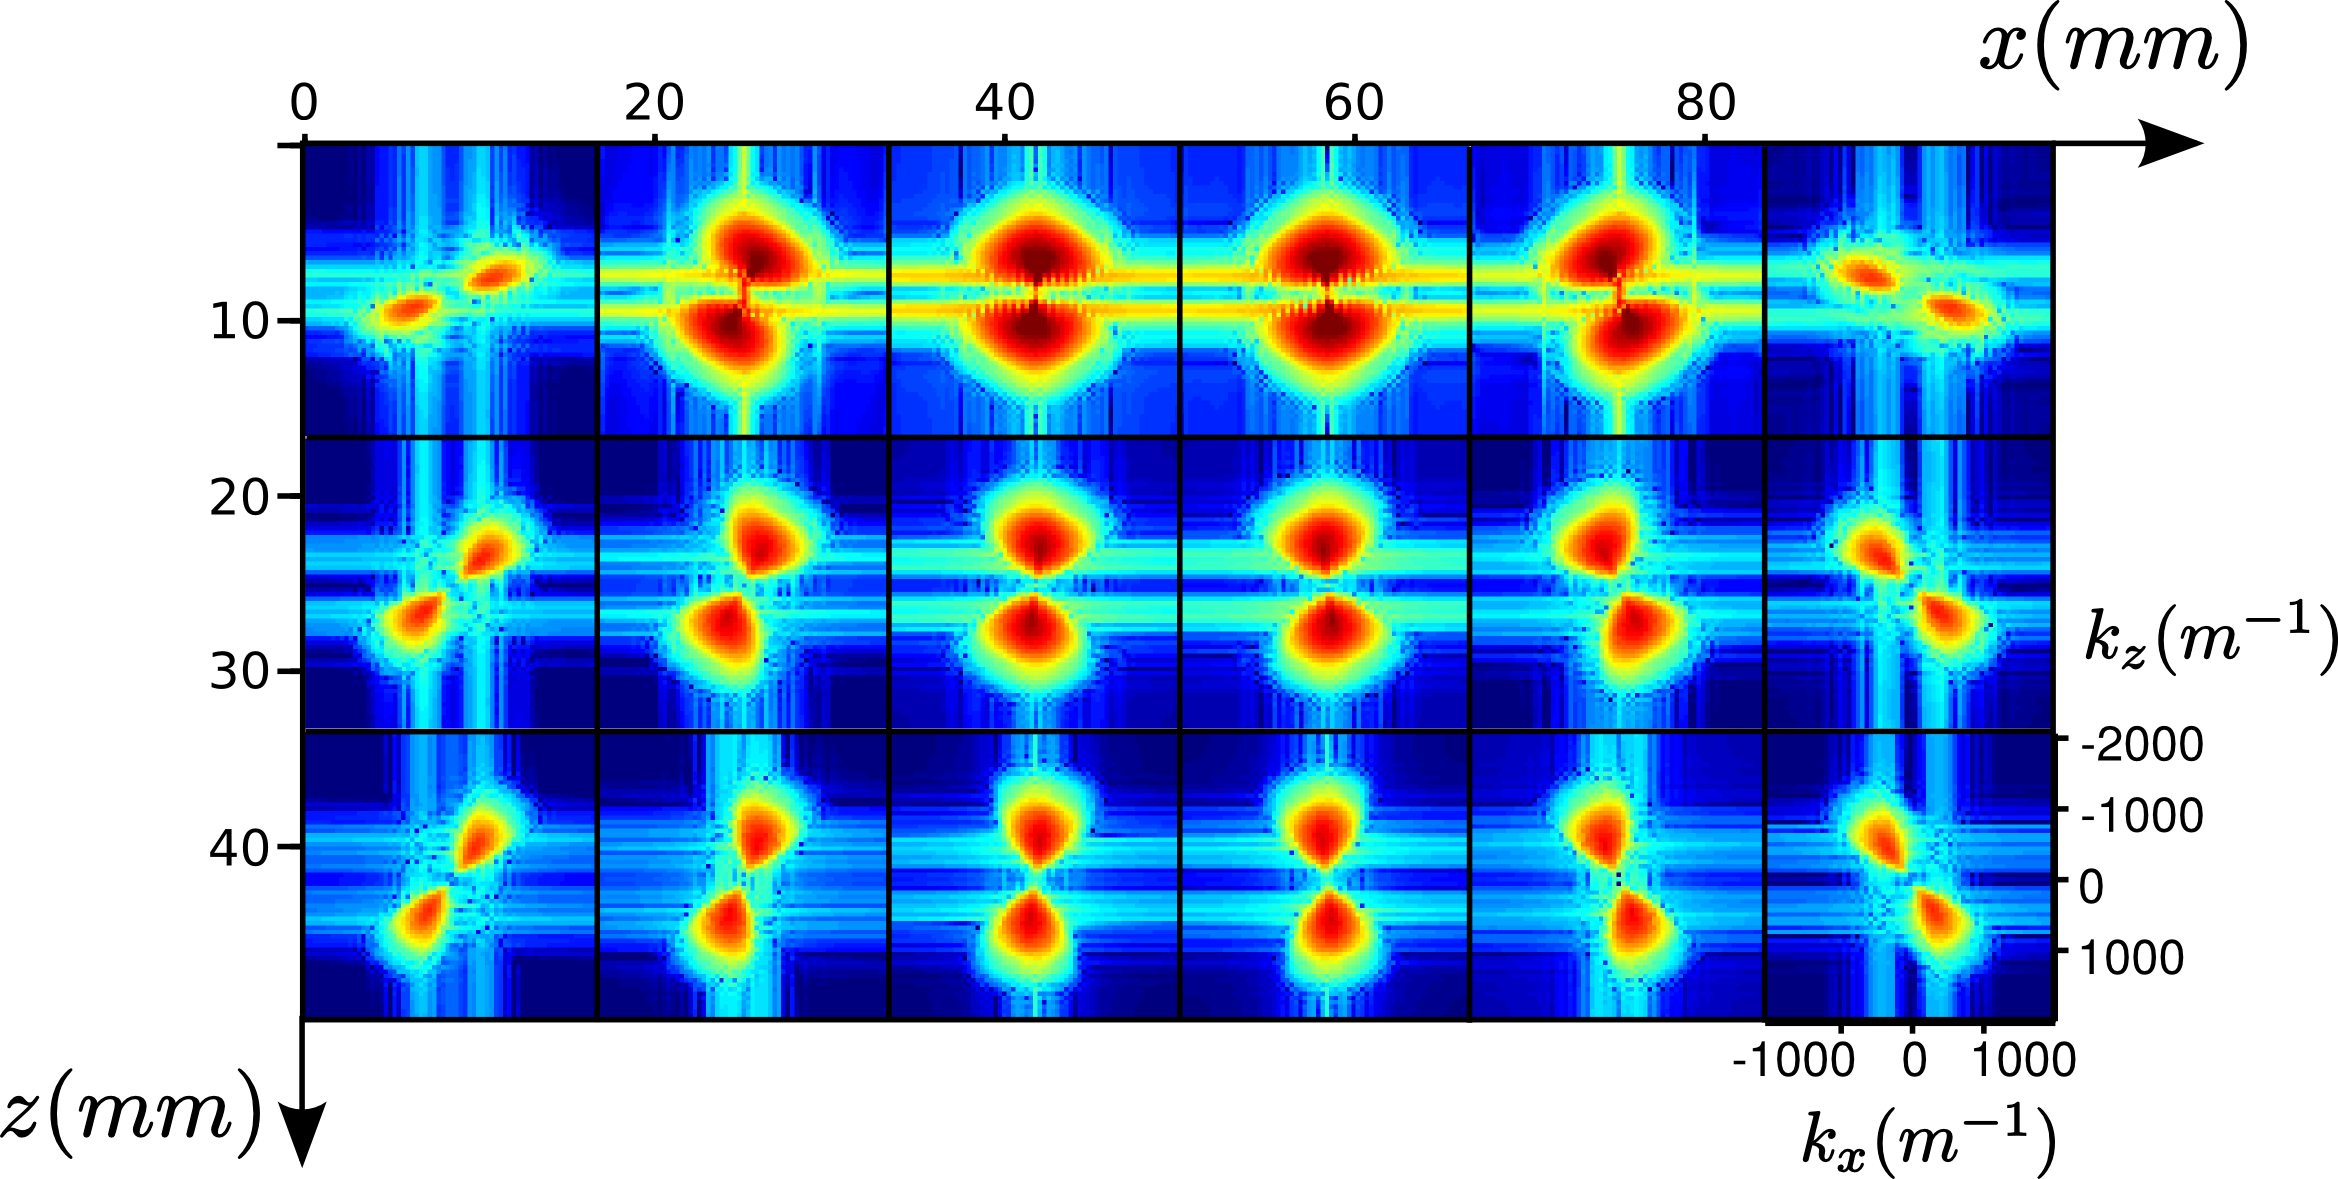
\includegraphics[width=1.5\textwidth]{img/ssfreesurf_2M}
		\caption{Excitation centrée à 2 MHz.}
		\label{app:2M}
	\end{subfigure}
	\caption{Transformées de Fourier spatiales locales pour 2 gammes de fréquence d'excitation.}
\end{figure}

Dans le cas d'une excitation basse fréquence, le gradient est pauvre en hauts nombres d'onde. Inversement, l'excitation haute fréquence ne permet pas de reconstruire les bas nombres d'onde.\\
La couverture en nombre d'onde est également très liée à l'acquisition. Elle est meilleure aux abords et en direction de la barrette. Les nombres d'onde verticaux seront globalement mieux reconstruits avec cette acquisition, tandis que la couverture en nombres d'ondes horizontaux est très faible.

\subsection{Influence des surfaces libres}


\section{Gestion des non-linéarités}
Une stratégie pour limiter la non-linéarité de l'inversion consiste à réaliser l'inversion en plusieurs temps, en injectant progressivement le contenu haute fréquence dans les données. L'inversion à basse fréquence permet ainsi de reconstruire la structure grossière avant d'ajouter les détails grâce à la résolution qu'offre le gradient en haute fréquence.\\



Afin que les nombres imagés soient correctement échantillonnés, il faut que le plus grand nombre d'onde imagé à une fréquence soit le même que que le plus petit à la fréquence suivante \citep{sirgue}. En considérant que le plus nombre d'onde est obtenu pour une angle de diffraction de $\pi/2$ , le rapport de fréquences suivant doit donc être respecté : 

\begin{alignat*}{3}
	  ~&k_{max}(f_{n}) &&= k_{min}(f_{n+1})\\
	\Leftrightarrow~~~~~ &  f_n &&= f_{n+1}\cos \left(\frac{\pi}{2} \right)\\
	 \Leftrightarrow~~~~~ & \frac{f_{n+1}}{f_n} && \approx  1,5.
\end{alignat*} 

Les inversions présentées ci-après sont donc réalisées en plusieurs itérations. Entre chaque itérations, les données observées et l'ondelette d'excitation sont filtrées par un filtre passe-bas de fréquence centrale $f_{n}$ et dont la fréquence de coupure haute est de $2,5 \times f_{n}$.


\section{Équations de propagation pour le problème direct}

La propagation des ondes élastiques est décrite par les équations linéarisées en déplacements $\bm{u}$ et contraintes $\bar{\bar T}$ suivantes \citep{mat_ac} : 

\begin{eqnarray}
	\rho \frac{\dd^2 u_{i}}{\dd t^2} &=& \displaystyle\sum_{j}\frac{\dd T_{ij}}{\dd x_{j}}\\
	T_{ij}&=&C_{ijkl}\left( \frac{\dd u_{i}}{\dd x_{j}} + \frac{\dd u_{j}}{\dd x_{i}}\right)\text{,}
	\label{prop}
\end{eqnarray}
avec $C_{ijkl}$ le tenseur des constantes élastiques.

\subsection{Propagation acoustique}
Les équations de la propagation acoustique peuvent être déduite de~\ref{prop} en considérant un module de cisaillement nul. on a alors $T_{ij}=0$ si $i\neq j$.

\subsubsection{Isotrope}
Dans un milieu isotrope, les constantes élastiques sont égales dans toutes les directions. En milieu acoustique isotrope, les propriétés élastiques sont donc réduites à une seule constante et les équations~\ref{prop} deviennent : 
\begin{eqnarray}
	\rho \frac{\dd^2 u_{i}}{\dd t^2} = -\bm{\nabla} p\\
	p=-\kappa \displaystyle\sum_{i} \frac{\dd u_{i}}{\dd x_{i}}\text{,}
\end{eqnarray}
avec $\kappa$ le module de rigidité et $p$ la pression.

\subsubsection{Transverse isotrope}

Il est possible de formuler à partir de~\ref{prop} des équations d'ondes acoustiques en milieu anisotrope. Bien que ce soit physiquement impossible, cette formulation permet de se rapprocher cinématiquement des équations d'ondes élastiques, de manière simplifiée \citep{alkhalifah}.

Notons que cette formulation [Pose quelques problèmes (Duveneck 2008) notamment génération d'onde S (sur données "vrai simulée"  et sur problème direct, mais pas la même car différente grille, PML, ... donc on la mute sur le résidu) qui n'a pas de sens physique. Proposer les solutions (taper Epsilon, en sismo on est dans l'eau donc c'est fait naturellement -> placer les sources dans un milieu isotrope).]
 

La paramétrisation du milieu est faite à l'aide des constantes de Thomsen~\citep{thomsen} surtout utilisées dans le domaine des Sciences de la Terre définies comme suit : 
\begin{eqnarray}
	\epsilon & =  & \frac{C_{11}-C_{33}}{2C_{33}} = \frac{\bm{v}_{p}.\bm{e}_{x} -  \bm{v}_{p}.\bm{e}_{z}}{\bm{v}_{p}.\bm{e}_{z}}\\
	\delta & = & \frac{(C_{13}+C_{44})^2-(C_{33}-C_{44})^2}{2C_{33}(C_{33-C_{44}})}\text{.}\\
\end{eqnarray}
+theta

Le paramètre $\epsilon$ est donc lié à la différence entre la composante verticale et la composante horizontale de la vitesse des onde de pression et $\delta$ décrit davantage la propagation des ondes quasi-longitudinales.



\section{Inversions en matériau acoustique }

Dans un premier temps, la méthode d'imagerie est appliquée à des milieux acoustiques, ce qui simplifie le problème et réduit les coût de calcul. Les études proposées dans cette section sont menées en approximation 2D : on suppose que le problème ne dépend pas du tout de la dimension données par $\bm{e}_{y}$.\\

Le code utilisé est \emph{TOYxDacTIME} développé dans le cadre du projet \emph{Seiscope}\footnote{http://seiscope2.osug.fr}. Le problème direct y est résolu par différences finies, ce qui contraint 

\subsection{Isotrope}




monoparamètre : vp
multi paramètre ?



\subsection{VTI}
Afin d'introduire une anisotropie simplifiée dans la soudure, une étude dans un milieu acoustique VTI est menée.\\

On considère une plaque isotrope dans laquelle se trouve une soudure anisotrope VTI sans défaut. On cherche à évaluer l'influence de l'anisotropie en vue d'inverser le paramètre $\epsilon$. La valeur de $\epsilon$ dans la soudure est fixée à 20\%, ce qui est environ deux fois plus élevé que les valeurs que l'on peut trouver dans la littérature~\citep{chassignole}. Les deux barrettes excitatrices/réceptrices sont placées de manière éloignée, afin d'accentuer la propagation des ondes suivant $\bm{e}_{x}$ et de s'assurer que les temps de vol soient perturbés par l'anisotropie (figure~\ref{configuration_vti}).\\
Les autres paramètres ($v_{p}$,$\rho$ et $\delta$) sont supposés constants et uniformes.\\

Une comparaison des données observées en milieu isotrope ($\epsilon = 0$) et avec la soudure anisotrope est proposée en figure~\ref{}. Il apparaît que la présence d'une anisotropie VTI a peu d'impact sur les données, car le dispositif d'acquisition favorise la mesure des ondes dont le trajet est majoritairement vertical et donc peu perturbé.\\
 L'inversion du paramètre $\epsilon$ est alors difficile : une modification grossière de la vitesse horizontale suffit à corriger les retards résiduels (cf figure~\ref{}).
 
 \todo[inline]{figures : configurations ; traces isotrope, epsilon=20 ; inversion + données calculées}
 
Un modèle de soudure anisotrope VTI est donc trop simple pour représenter l'anisotropie d'une soudure réelle, dont on sait qu'elle impacte beaucoup le faisceau ultrasonore. Pour tester la capacité de la FWI à reconstruire ces paramètres d'anisotropie, il est donc nécessaire d'utiliser un modèle plus pertinent qui se rapprocherait davantage de celui proposé par \cite{ogilvy} par exemple.\\

Le modèle proposé par \cite{ogilvy} est de la forme : 
\begin{equation}
	\theta(x,z) = \tan^{-1}\left( \frac{D/2 + z\tan\alpha}{x} \right),
\end{equation}
avec $D$ la largeur de la racine de la soudure et $\alpha$  l'angle du bord de soudure.

 Conclusion : inversion de $\epsilon$ -> dur et par pertinent
passer en tilted (façon ogilvy ?) ou modèle plus précis en élastique.

\section{Inversions en matériau élastique isotrope}




%%%%%%%%%%%%%%%%%%%%%notes%%%%%%%%%%%%%%%
\todo[inline]{notes : }
\subsection{anisotrope}

anisotrope est plus problématique que isotrope car : 
-modélisation plus complexe,
-problème moins bien posé

Gholami 2011 : la vitesse a beaucoup plus d'influence sur les données que les paramètres delta et epsilon (delta étant le plus faible). D'après ses schémas, on va donc avoir une maj de la vitesse mais pas des autres paramètres

modèle initial de soudure : citer mina ?

%VTI elliptique ne gène pas l'inversion car beaucoup d'info portées par la transmission (vecteurs d'ondes verticaux non affectés par l'anisotropie elliptique VTI)  -> pas assez proche du modèle réel

%le flop du vti montre que l'inversion des paramètres est tributaire de l'acquisition

Romain : passer en TTI (code en freq)



%\addcontentsline{toc}{section}{\textbf{Annexe}}

\chapter{Inversion à partir d'une acquisition réaliste \label{annexe:acqui}}
Un exemple d'inversion monoparamètre de la vitesse est présenté ici, à partir d'une acquisition qui n'est pas en contact avec le relief de la soudure. Deux barrettes de 64 éléments espacées de 1 mm sont placées de chaque côté de la racine de la soudure. Les données sont générée à partir d'une soudure de densité uniforme d'une valeur de 8000 kg/m$^{3}$ et de vitesse présentée en figure~\ref{app:iso:reel1}. La durée des signaux acquis est de 30.7 $\mu s$, ce qui est le temps nécessaire à la propagation d'une extrémité à l'autre du système d'acquisition. Le modèle initial de vitesse est uniforme, avec $v_{p}=6000$~m/s. Le modèle pour la masse volumique est fixé à sa valeur vraie.\\

 Le résultat de l'inversion, réalisée sur des fréquences allant de 200 k à 5 MHz, est présenté en figure~\ref{app:iso:reel2}. Il illustre à nouveau la dépendance de la résolution vis à vis du système d'acquisition. En effet, la racine de la soudure est mal reconstruite dans cette zone car les diffractions mesurées sont d'angle nul ou proche de $\pi$. Or, les angles de diffraction proches de $\pi$  contribuent à une reconstruction de résolution très faible, d'après l'expression du nombre d'onde~\ref{app:nb_onde}. Pour une application de la FWI à un cas réel, il est donc nécessaire de déterminer au préalable l'acquisition favorisant un éclairage adapté à la géométrie de la pièce à évaluer.
 
\begin{figure}[!h]
	\begin{subfigure}[b]{0.5\textwidth}
		\centering
		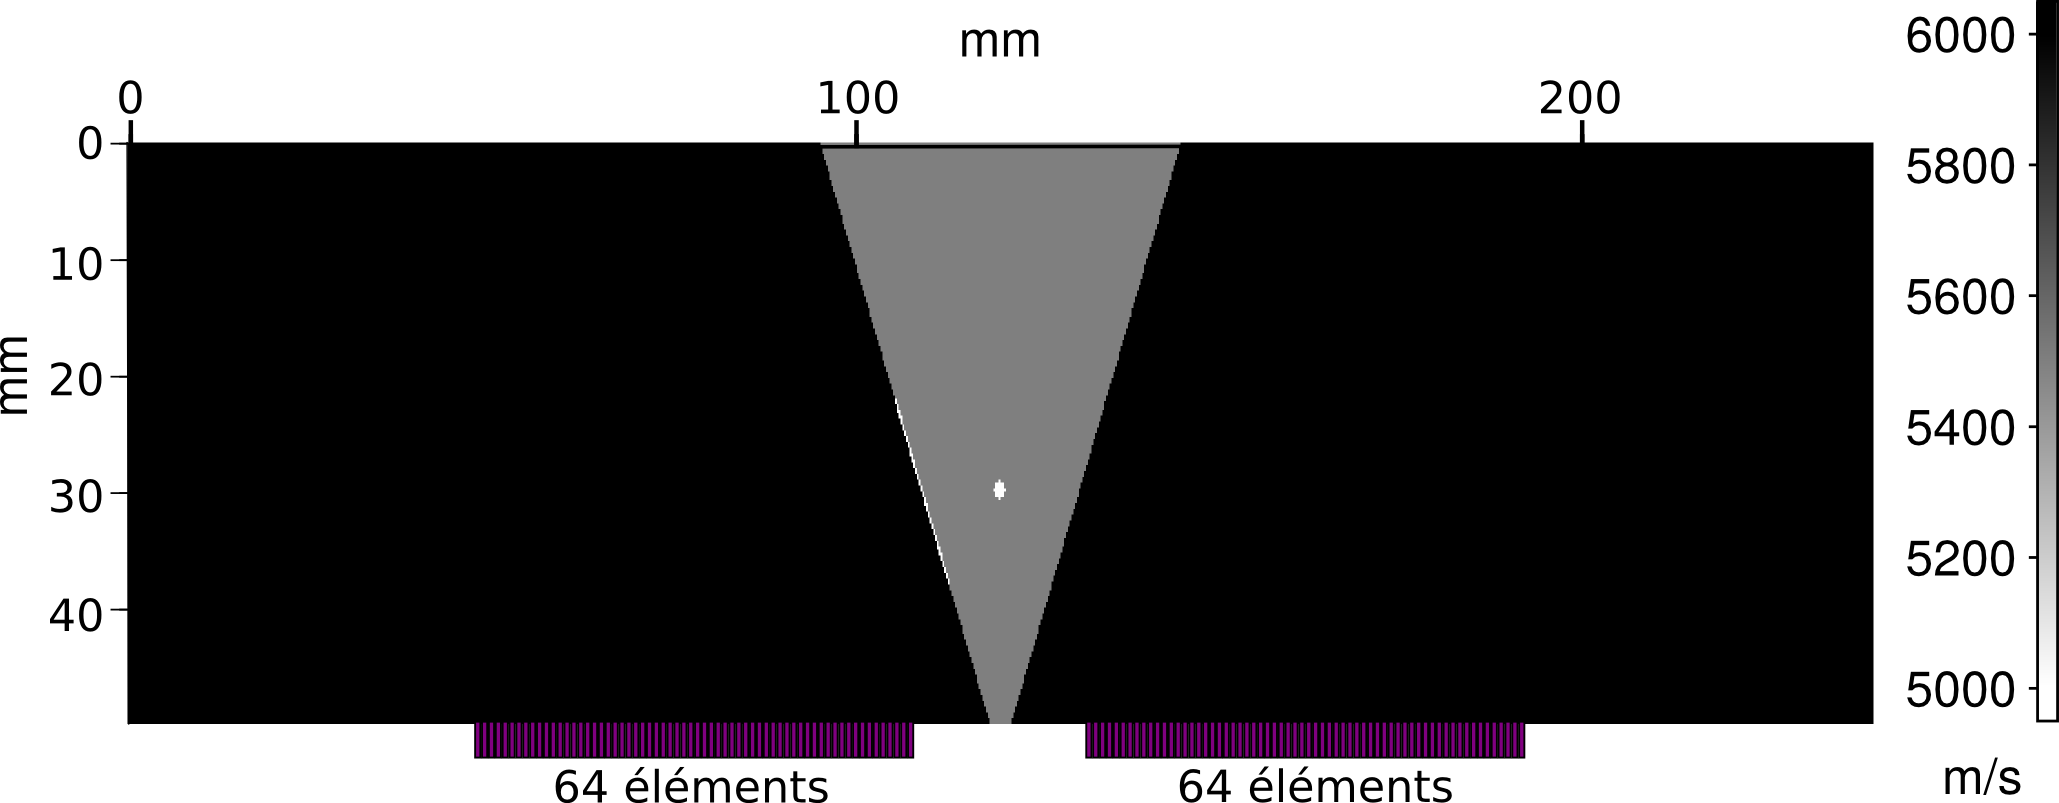
\includegraphics[width=\textwidth]{img/config_reelle_true.png}
		\caption{Configuration du système d'acquisition et vitesse utilisée pour la génération des données.\label{app:iso:reel1}}	
	\end{subfigure}
	\hspace{0.2cm}
	\begin{subfigure}[b]{0.5\textwidth}
		\centering
		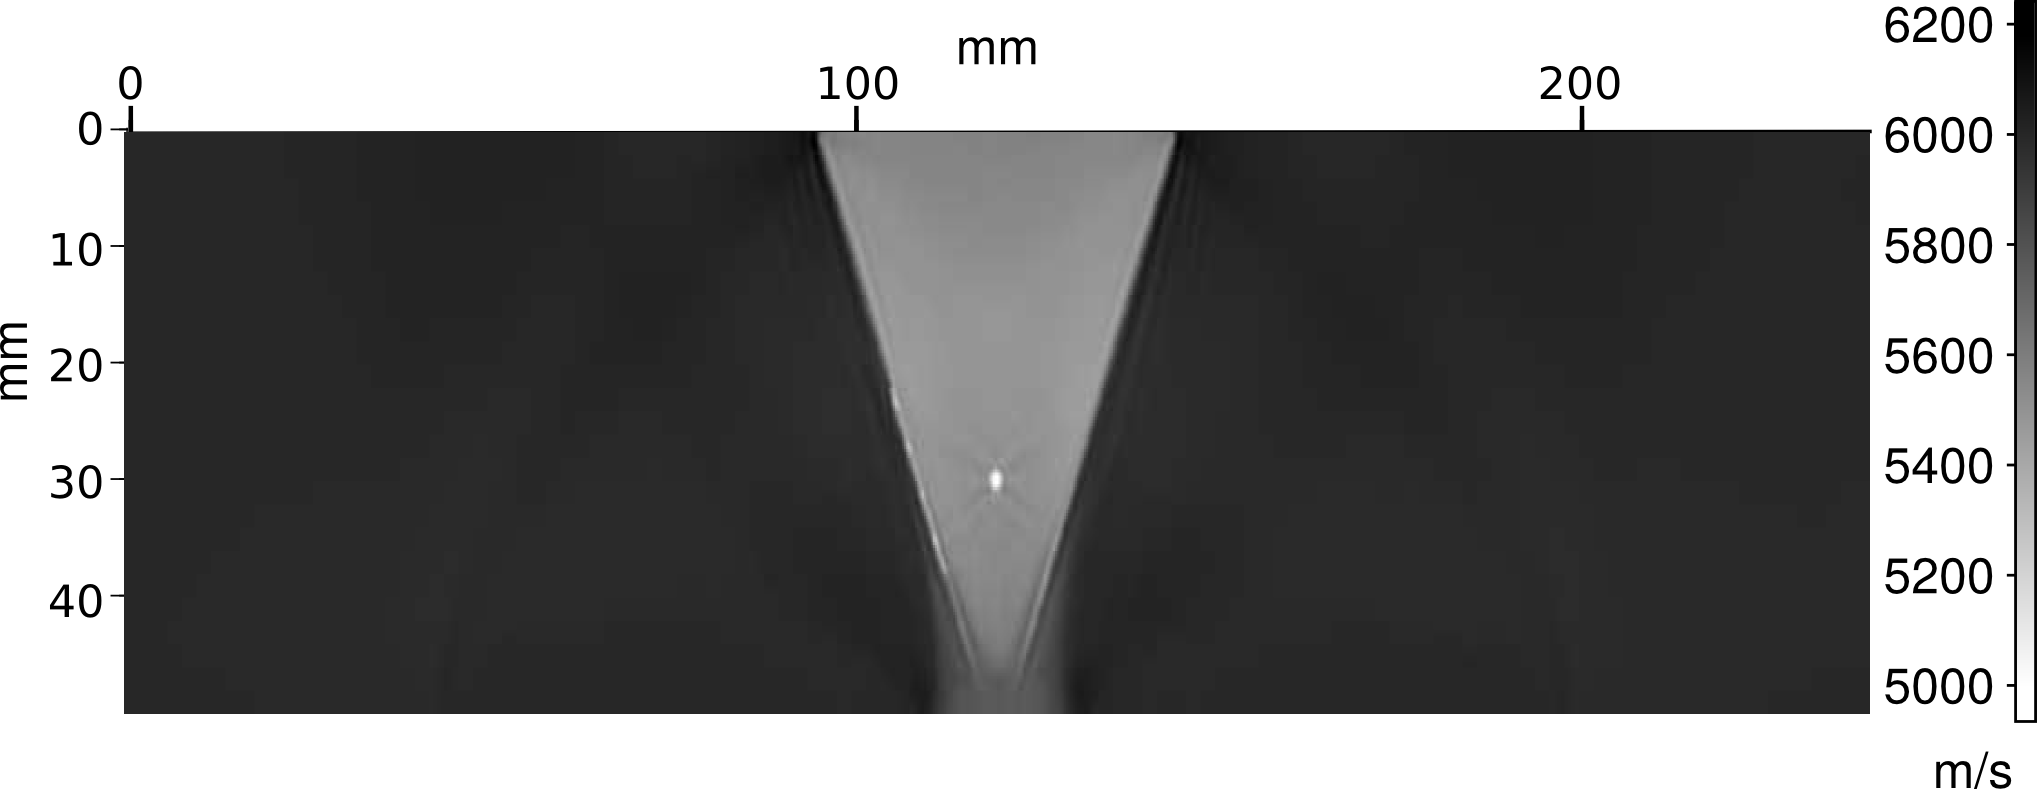
\includegraphics[width=\textwidth]{img/config_reelle_rec.png}
		\caption{Vitesse reconstruite par inversion monoparamètre. \label{app:iso:reel2}}	
	\end{subfigure}
	\caption{Exemple d'inversion pour une acquisition unilatérale. Chaque barrette est utilisée en excitation et en réception.}
\end{figure}



\chapter{Discrétisations et ressources nécessaires à l'inversion \label{annexe:chiffres}}

\section*{Discrétisation spatiale}
La résolution du problème direct par différences finies d'ordre 4 en espace sur maillage décalé nécessite de prendre un pas de discrétisation spatiale d'au moins 5 points par longueur d'onde \citep{levander}, afin de limiter la dispersion numérique.\\

Considérant que la plus petite longueur d'onde propagée est à 4 MHz, pour une vitesse minimale des ondes de compression de 5000 m/s, le pas de discrétisation spatiale choisi pour la propagation des ondes en milieu acoustique est $\Delta x=0,25$~mm.

\section*{Discrétisation temporelle}

Considérant un schéma à l'ordre 2 en temps et un espace à 2 dimensions, \cite{levander} préconise de respecter le critère de stabilité  
\begin{equation}
	\Delta t \leq \frac{\Delta x}{(c_{1}+c_{2})\sqrt{2} c_{max}},
\end{equation}
avec $c_{1}=\nicefrac{1}{24}$ et $c_{2}=\nicefrac{9}{8}$. En considérant une vitesse maximale de 6500 m/s et avec le pas de discrétisation spatiale choisi précédemment, il faut donc que 

\begin{equation}
	\Delta t \leq 2,3.10^{-8} \text{~s.}
\end{equation}
Respectant cette condition, la discrétisation spatiale utilisée pour tous les calculs de problème direct de cette étude est $\Delta t=1,5.10^{-8}$~s.



\section*{Ressources numériques}

Les inversions présentées dans ce rapport sont le résultats d'une suite d'inversions réalisées successivement à partir des données de références filtrées dans 9 gammes de fréquences, allant de 100 k à 3,4 MHz. 9 inversions sont donc réalisées, comportant chacune 20 perturbations successives du modèle.\\

Les calculs ont été réalisé sur les machines du centre de calcul CIMENT \footnote{Calcul Intensif / Modélisation / Expérimentation Numérique et Technologique : https://ciment.ujf-grenoble.fr}. Le temps de calcul nécessaire à une inversion (pour une seule gamme de fréquence) à 128 sources, est d'environ 5 minutes sur 128 cœurs  (sur des nœuds constitués de 8 biprocesseurs\footnote{d'architecture Sandy Bridge, Intel}, soit 16 cœurs par nœud).\\

 À titre de comparaison,  le calcul TFM prend une dizaine de minutes sur un ordinateur personnel\footnote{2 coeurs, 4 threads (processeur i7-4600u, Intel)} (pour une discrétisation spatiale semblable à celle utilisée pour la FWI).




%\section{Note sur les dimensions des grandeurs du chapitre \ref{fwi}}
%
%Les matrice $A$, qui est l'opérateur de l'équation d'onde a les dimensions de l'espace du problème direct : $l\times l$, où $l=n_{x}\times n_{z}$, $n_{x}$ et $n_{z}$ étant les dimensions du milieu de propagation discrétisé.\\
% De la même façon, le champ d'onde $\bm{u}$ et le vecteur source $\bm{s}$ sont de dimension $l\times 1$.\\
%Or, les vecteurs de données $\bm{d}$ ne contiennent que les informations aux $n$ points de réception. Ils sont donc de dimension $1\times n$. Les calculs sont donc menés sur des vecteurs agrandis à l'aide de zéros de façon à ce que $\bm{d}$ soit de dimension $l\times 1$. \\
%Finalement, le gradient  $\frac{\dd C (\bm{m})}{\dd \bm{m}}$ est bien de dimension $M\times 1$ avec $M$ le nombre de paramètre du problème \citep{pratt_98}.



%%%%%%%% Biblio %%%%%%%%%%
\newpage

\bibliographystyle{plainnat}%\bibliographystyle{unsrt}
\bibliography{biblio}

\end{document} % fin doc


